\documentclass[11pt,letterpaper]{article}

%\usepackage{fontspec}
%\usepackage[utf8]{inputenc}
\usepackage{textcomp,marvosym}
\usepackage{amsmath,amssymb}
\usepackage[normalem]{ulem}
\usepackage[left]{lineno}
\usepackage{booktabs}
\usepackage{changepage}
\usepackage{rotating}
\usepackage{color}
\usepackage{natbib}
\usepackage{setspace}
\usepackage{array}
\usepackage{fancyhdr}
\usepackage{graphicx}
\usepackage{sidecap}
\usepackage{xspace}
\usepackage[hidelinks]{hyperref}
\urlstyle{same}
\usepackage{threeparttable}
%\doublespacing

\newcommand{\mitbf}[1]{\hbox{\mathversion{bold}$#1$}}

\raggedright
\textwidth = 6.5 in
\textheight = 8.25 in
\oddsidemargin = 0.0 in
\evensidemargin = 0.0 in
\topmargin = 0.0 in
\headheight = 0.0 in
\headsep = 0.5 in
\parskip = 0.1 in
\parindent = 0.2in

\usepackage[aboveskip=1pt,labelfont=bf,labelsep=period,justification=raggedright,singlelinecheck=off,font=small]{caption}

\pagestyle{myheadings}
\pagestyle{fancy}
\fancyhf{}
\lhead{Bayesian inversion for paleogeographic reconstruction}
\rhead{\thepage}

\begin{document}

\begin{flushleft}
{\Large \textbf{Bayesian inversion for paleogeographic reconstruction}}

Ian R. Rose\textsuperscript{1},
Yiming Zhang\textsuperscript{1},
Nicholas L. Swanson-Hysell\textsuperscript{1}\textsuperscript{*}

\bigskip
\textsuperscript{1} Department of Earth and Planetary Science, University of California, Berkeley, CA, USA\\
\textsuperscript{*} Correspondence to: Nicholas L. Swanson-Hysell, swanson-hysell@berkeley.edu
\bigskip

\end{flushleft}

\noindent\textit{This manuscript is in preparation for submission to Journal of Geophysical Research: Solid Earth.}

\linenumbers

\section*{Abstract \label{sec:ABSTRACT}}

Apparent polar wander paths (APWPs) synthesized from paleomagnetic poles provide the most direct data for reconstructing past paleogeography and plate motions for times earlier than $\sim$200 Ma. However, it can be difficult to develop and interpret APWPs in the presence of errors on pole positions, age uncertainties, and the lack of paleolongitude control associated with individual paleomagnetic poles. Approaches for dealing with the uncertainties and compiling paleomagnetic poles into APWPs for continental blocks include the development of running mean averages and the fitting of spherical splines to pole positions. In this contribution, we describe a new method for APWP synthesis from paleomagnetic poles. The approach extends the paleomagnetic Euler pole analysis of \citet{Gordon1984a} by placing it within the framework of a Bayesian inverse problem. This approach allows uncertainties in both pole position and age to be incorporated into the synthesis -- uncertainties that are often ignored in standard treatments. The paleomagnetic Euler poles resulting from the inversion provide estimates for the total plate motions (not just the latitudinal components) as well as their uncertainties. In addition to estimating a single Euler pole, the method allows for changepoints from one Euler pole to another to be solved for as part of the inversion. The inversion path can be restricted to be a great circle therefore allowing inversion for true polar wander or true polar wander in combination with small circle paths associated with plate tectonic motion. We show several example inversions on simple synthetic data to demonstrate the capabilities of the method. We illustrate application of the method to constrain rapid rates of motion for cratonic North American associated with the Keweenawan Track of late Mesoproterozoic paleomagnetic poles. We also apply the method to the Cenozoic database of Australia paleomagnetic poles which can be compared to independent plate reconstrucions. That the computational power to use Markov chain Monte Carlo methods to estimate paleomagnetic Euler poles has to the potential to open new directions in quantitative paleogeography.

\section*{Introduction}

Plate tectonics is the motion of near-rigid blocks of lithosphere across the surface of Earth, separated by relatively narrow regions of deformation in spreading centers, transform faults, and subduction zones. The rigidity of plates means that the motion of most of Earth's surface can be described by a set of Euler poles which specify the position (in latitude and longitude) of a rotation axis and and rate of rotation about this axis for a given plate \citep[cf.][]{Cox2009a}. Individual points on a plate undergoing rigid rotation are described by small circle paths.

Euler poles are widely used for describing plate motions due to their simplicity and compactness \citep[e.g.][]{DeMets2010a, Argus2011a}. Given that it takes time to build up and change torques that drive plate motions, plate motions have a tendency to remain constant, or approximately so, over time scales of millions to tens of millions of years \citep{Iaffaldano2012a}. This consistency of motion can be seen physically expressed in the shape of oceanic fracture zones and in hotspot tracks across the lithosphere. These features form gently curving arcs over large portions of Earth's surface that can be well described by small circles, consistent with finite Euler rotations of the plate for an extended period of time. As such, the combination of an Euler pole plus a time interval for which it is active (often called a ``stage pole'') is a convenient description of plate motions through Earth history.

As the stage pole description of plate motions is a convenient way of reconstructing plate tectonic history, it is widely used in both continental reconstruction \citep[e.g.][]{Boyden2011a} and in geodynamical modeling \citep[e.g.][]{Mcnamara2005a, Bull2014a}. Most reconstructions of plate motions over the past 200 million years rely heavily on fitting Euler pole rotations to oceanic fracture zones, hotspot tracks, seafloor magnetic isochrons, and, to a lesser extent, paleomagnetic data \citep{Muller1993a, Seton2012a}. However, as we look further back in Earth history, many of the records on which these plate tectonic reconstructions rely largely disappear due to the  subduction of oceanic lithosphere. Given the lack of ocean crust older than $\sim$200 Ma, the paleomagnetic record from continental rocks is the dominant remaining evidence. These paleomagnetic data can be used in conjunction with geological data that provides information on the tectonic setting of plate margins, as well as additional information such as the correlation of geologic terranes, to develop paleogeographic reconstructions.

% \begin{figure}[h!]
% \begin{center}
% 	\includegraphics[width=0.9\textwidth]{./Figures/Continent_Areas.pdf}
% 	\caption{\textbf{A)} Total continental area through time. In the paleogeographic model used in this study, tectonic units \citep{Torsvik2016a} are progressively added to the model, leading to a net increase in total continental area in the model of $\sim$33\% over the Phanerozoic. However, estimates of continental crust growth (e.g. \citealp{Pujol2013a}) suggest that continental area was roughly constant through the Phanerozoic. We therefore normalize the total continental area curve in our model by assuming a fixed continental area through the Phanerozoic. \textbf{B)} Tropical continental area through time. We normalize the tropical continental area curve using the normalization ratio implied in (A). \textbf{C)} Contour plot showing the latitudinal distribution of continental area. \textbf{D)} Latitudinal extent of land ice away from the poles \citep{Macdonald2019a}.}
% 	\label{fig:Continent_Areas}
% \end{center}
% \end{figure}

It is more challenging to reconstruct past plate motions from the paleomagnetic record than from data derived from oceanic lithosphere for a number of reasons, including: (1) the data are often sparser; (2) traditional paleomagnetic analysis constrains paleolatitude and the orientation of a continental block, but does not constrain paleolongitude without additional assumptions; and (3) some paleomagnetic poles have poor age control.

\citet{Gordon1984a} noted that apparent polar wander paths (APWPs) have arcing trajectories similar to fracture zones and hotspot tracks, which is to be expected if similar tectonic processes are responsible for creating them. They therefore suggested fitting small circles to paleomagnetic poles tracks, which would furnish Euler poles for the plate in question for that time period. This approach for constraining APWPs, called paleomagnetic Euler pole (PEP) analysis, has the attractive feature of providing a complete description of the plate motion, including paleolongitudinal changes and speeds.  However, it has the drawback of not providing readily computed uncertainties associated with the fit and not incorporating age uncertainties. With some notable exceptions \citep[e.g.][]{Bryan1986a, Beck1989a, Tarling1996a, Beck2003a, Smirnov2010a}, PEP analysis has not seen wide adoption.

In this contribution, we extend paleomagnetic Euler pole (PEP) analysis by placing it within a Bayesian statistical framework, and demonstrate how to invert for PEPs using Markov chain Monte Carlo (MCMC) methods. This framework has the advantage of naturally incorporating uncertainties in paleomagnetic pole positions, as well as widely disparate age uncertainties associated with individual paleomagnetic poles. The resulting stage poles from these inversions are not a single answer, but are instead a distribution of possible answers, furnishing uncertainties as part of the solution process. \citet{Iaffaldano2012a} employed a similar Bayesian approach to inversions for finite plate rotations. They used seafloor data to reconstruct India's Cenozoic convergence with Asia, incorporating uncertainties into the inversion. In the process, they demonstrated that interpretations of changes in plate motions on timescales $<$1 Myr are the result of overfitting of data and there are fewer kinematic changes and longer stability in plate motions than previous treatments.

In this contribution, we first review different approaches that have been applied to synthesize and interpret APWPs. We then describe the formalism of Bayesian inversions and Markov chain Monte Carlo methods that we will apply. We then describe the statistical model which we will be inverting and demonstrate the inversion of several synthetic data sets. We then show examples where we apply the method to paleomagnetic poles in order to develop estimates of paleomagnetic Euler pole positions and obtain estimates of plate velocity.

\section*{Interpretation of apparent polar wander paths}

A sequence of paleomagnetic poles from the same continental block can be synthesized into an APWP, which can then be used to develop plate tectonic reconstructions and models of plate speeds through time. Interpretation of these paths becomes difficult in the case of limited, uncertain, or conflicting data, and when the age of paleomagnetic poles are poorly known. A number of approaches to dealing with uncertainty in APWPs have been developed, which we briefly review here.

\subsection*{Latitudinal drift}
Due to the rotational symmetry of Earth's time-averaged geocentric axial dipole magnetic field, paleomagnetic poles do not directly constrain the absolute paleolongitude of a lithospheric block \citep{Butler1992a}. The simplest analysis of an APWP is thus to compare the paleolatitudes implied by successive poles for a point on a respective block. The difference in paleolatitudes gives a minimum angular distance over which the block has traveled.  When this distance is compared to the age difference between the poles, such a comparison establishes a rate of latitudinal motion.

It is possible to estimate confidence bounds on the rate of latitudinal drift through bootstrap resampling \citep[e.g.][]{Tarduno1990b} or by taking a Monte Carlo approach. \citet{Swanson-Hysell2014b} developed a Monte Carlo sampling method and applied the method to a pair of poles from the Proterozoic Midcontinent Rift of North America to estimate the range of implied latitudinal drift. They also sampled from the uncertainties of radiometric dates associated with the poles, assuming Gaussian distributions, in order to incorporate age uncertainties into the analysis. With samples of pole position and ages, they were able to estimate the 95\% confidence estimates on the rate of latitudinal drift.

Whether using point estimates of the latitudinal drift rate or using Monte Carlo estimates, the latitudinal drift interpretation of APWPs remains limited as it represents a minimum estimate. It does not resolve longitudinal drift rate, nor does it naturally extend to APWPs with more than two poles, especially if two coeval poles are not in agreement, as it requires the selection of pole pairs.

\subsection*{Spherical splines}
When considering APWPs with many poles, it becomes more difficult to perform latitudinal comparisons between pairs of poles. It is not always clear which pairs of poles to compare in cases where there are many overlapping paleomagnetic poles, that have variable uncertainities associated with their position and age.

One approach to synthesize such data is to fit a spline through the set of paleomagnetic poles, constraining the path to lie on the surface of a sphere. This approach was pioneered by \citet{Torsvik1992a} using the spherical spline algorithm developed by \citet{Jupp1987a}. This approach has the advantage of allowing the weighting of the data by their uncertainties. The uncertainty assigned to a paleomagnetic pole can be the 95\% confidence interval on the pole, but it can also be augmented by various quality screening factors, such as the quality (``Q'') factor of \citet{Van-der-Voo1990a} \citep{Torsvik1992a}. Even with the weighting of the paleomagnetic poles by uncertainty there can be unrealistic loops in the APWP generated by the spline fit. To combat this, the spline can also be computed under tension, penalizing curvature and producing a smoother path \citep{Torsvik1996a}.

The spherical spline approach to interpreting APWPs has several attractive features. It produces a smooth path through the data that can incorporate spatial uncertainties in the data, and may be efficiently computed. However, it does have some drawbacks. It is not easy to determine the appropriate uncertainty weighting and spline tension parameters for the fit, and what effect those choices have on the result. Furthermore, the resulting fit does not have an uncertainty with a physically interpretable meaning \citep{Torsvik1996a}. It also does not have a simple way of incorporating age uncertainties of the paleomagnetic poles. Finally, by their very nature, splines cannot represent the sharp hairpin cusps that characterize abrupt shifts in motion that plates sometimes undergo \citep{Irving1972a, Gordon1984a}.

\subsection*{Running means}

An alternative method for developing APWPs is to perform a running Fisher mean on the poles with a moving window \citep{Irving1977a, Van-der-Voo2001a, Torsvik2008a}. In such an analysis, paleomagnetic poles in a compilation are averaged in defined steps (typically 5-10 Myr) with a defined window duration (typically 10-30 Myr). Like spherical splines, the running mean approach has the ability to effectively damp the effect of outlier poles that could lead to spurious motion in the APWP if there are sufficient data. The duration of the moving window controls the amount of smoothing. Furthermore, this moving window method enforces an age progression in the averaged poles. \citet{Torsvik2008a} also investigated the effects of combining running means with spherical splines, by first computing a set of mean poles and then fitting a spline through those means. 
The simplicity of using the running mean approach to develop an APWP, as well as its ability to suppress potentially spurious poles, has led to it being widely adopted.

The running mean approach shares many of the drawbacks of the spline approach.  It is not obvious how to best choose the window duration, and different window durations are likely appropriate for different data sets.  It is also unclear how to interpret the resulting uncertainties in the path that are reported as the Fisher $A_{95}$ ellipse of the mean of the poles. This approach, along with the spherical spline method, does not easily incorporate age uncertainties in the poles, nor the uncertainty in pole positions.

\subsection*{Paleomagnetic Euler poles}
The idea of fitting small circles to paleomagnetic data to gain insight into plate motions was first described by \citet{Francheteau1969a}. The center of such a circle on a sphere is the pole of rotation which was termed a paleomagnetic euler pole (PEP) by \citet{Gordon1984a} who developed a method to invert for the position of such poles. The approach builds on the recognition that plate motions are well described by finite rotations around Euler poles which are approximately steady for millions or tens of millions of years. As a result, the APWP of a plate can be described by Euler rotations, which produce small circle paths on Earth's surface. As a result, PEP analysis conforms to the general model of the movement of tectonic plates. Since the analysis solves for the Euler pole that produces a given small circle, this approach allows for an estimate of the full motion of a given plate, including the total plate speed (instead of just the latitudinal component of the speed). Effectively, the analysis utilizes both the change in plate orientation and latitude embedded within paleomagnetic poles to estimate both latitudinal and longitudinal motion as succinctly summarized by an Euler pole.

\begin{SCfigure}
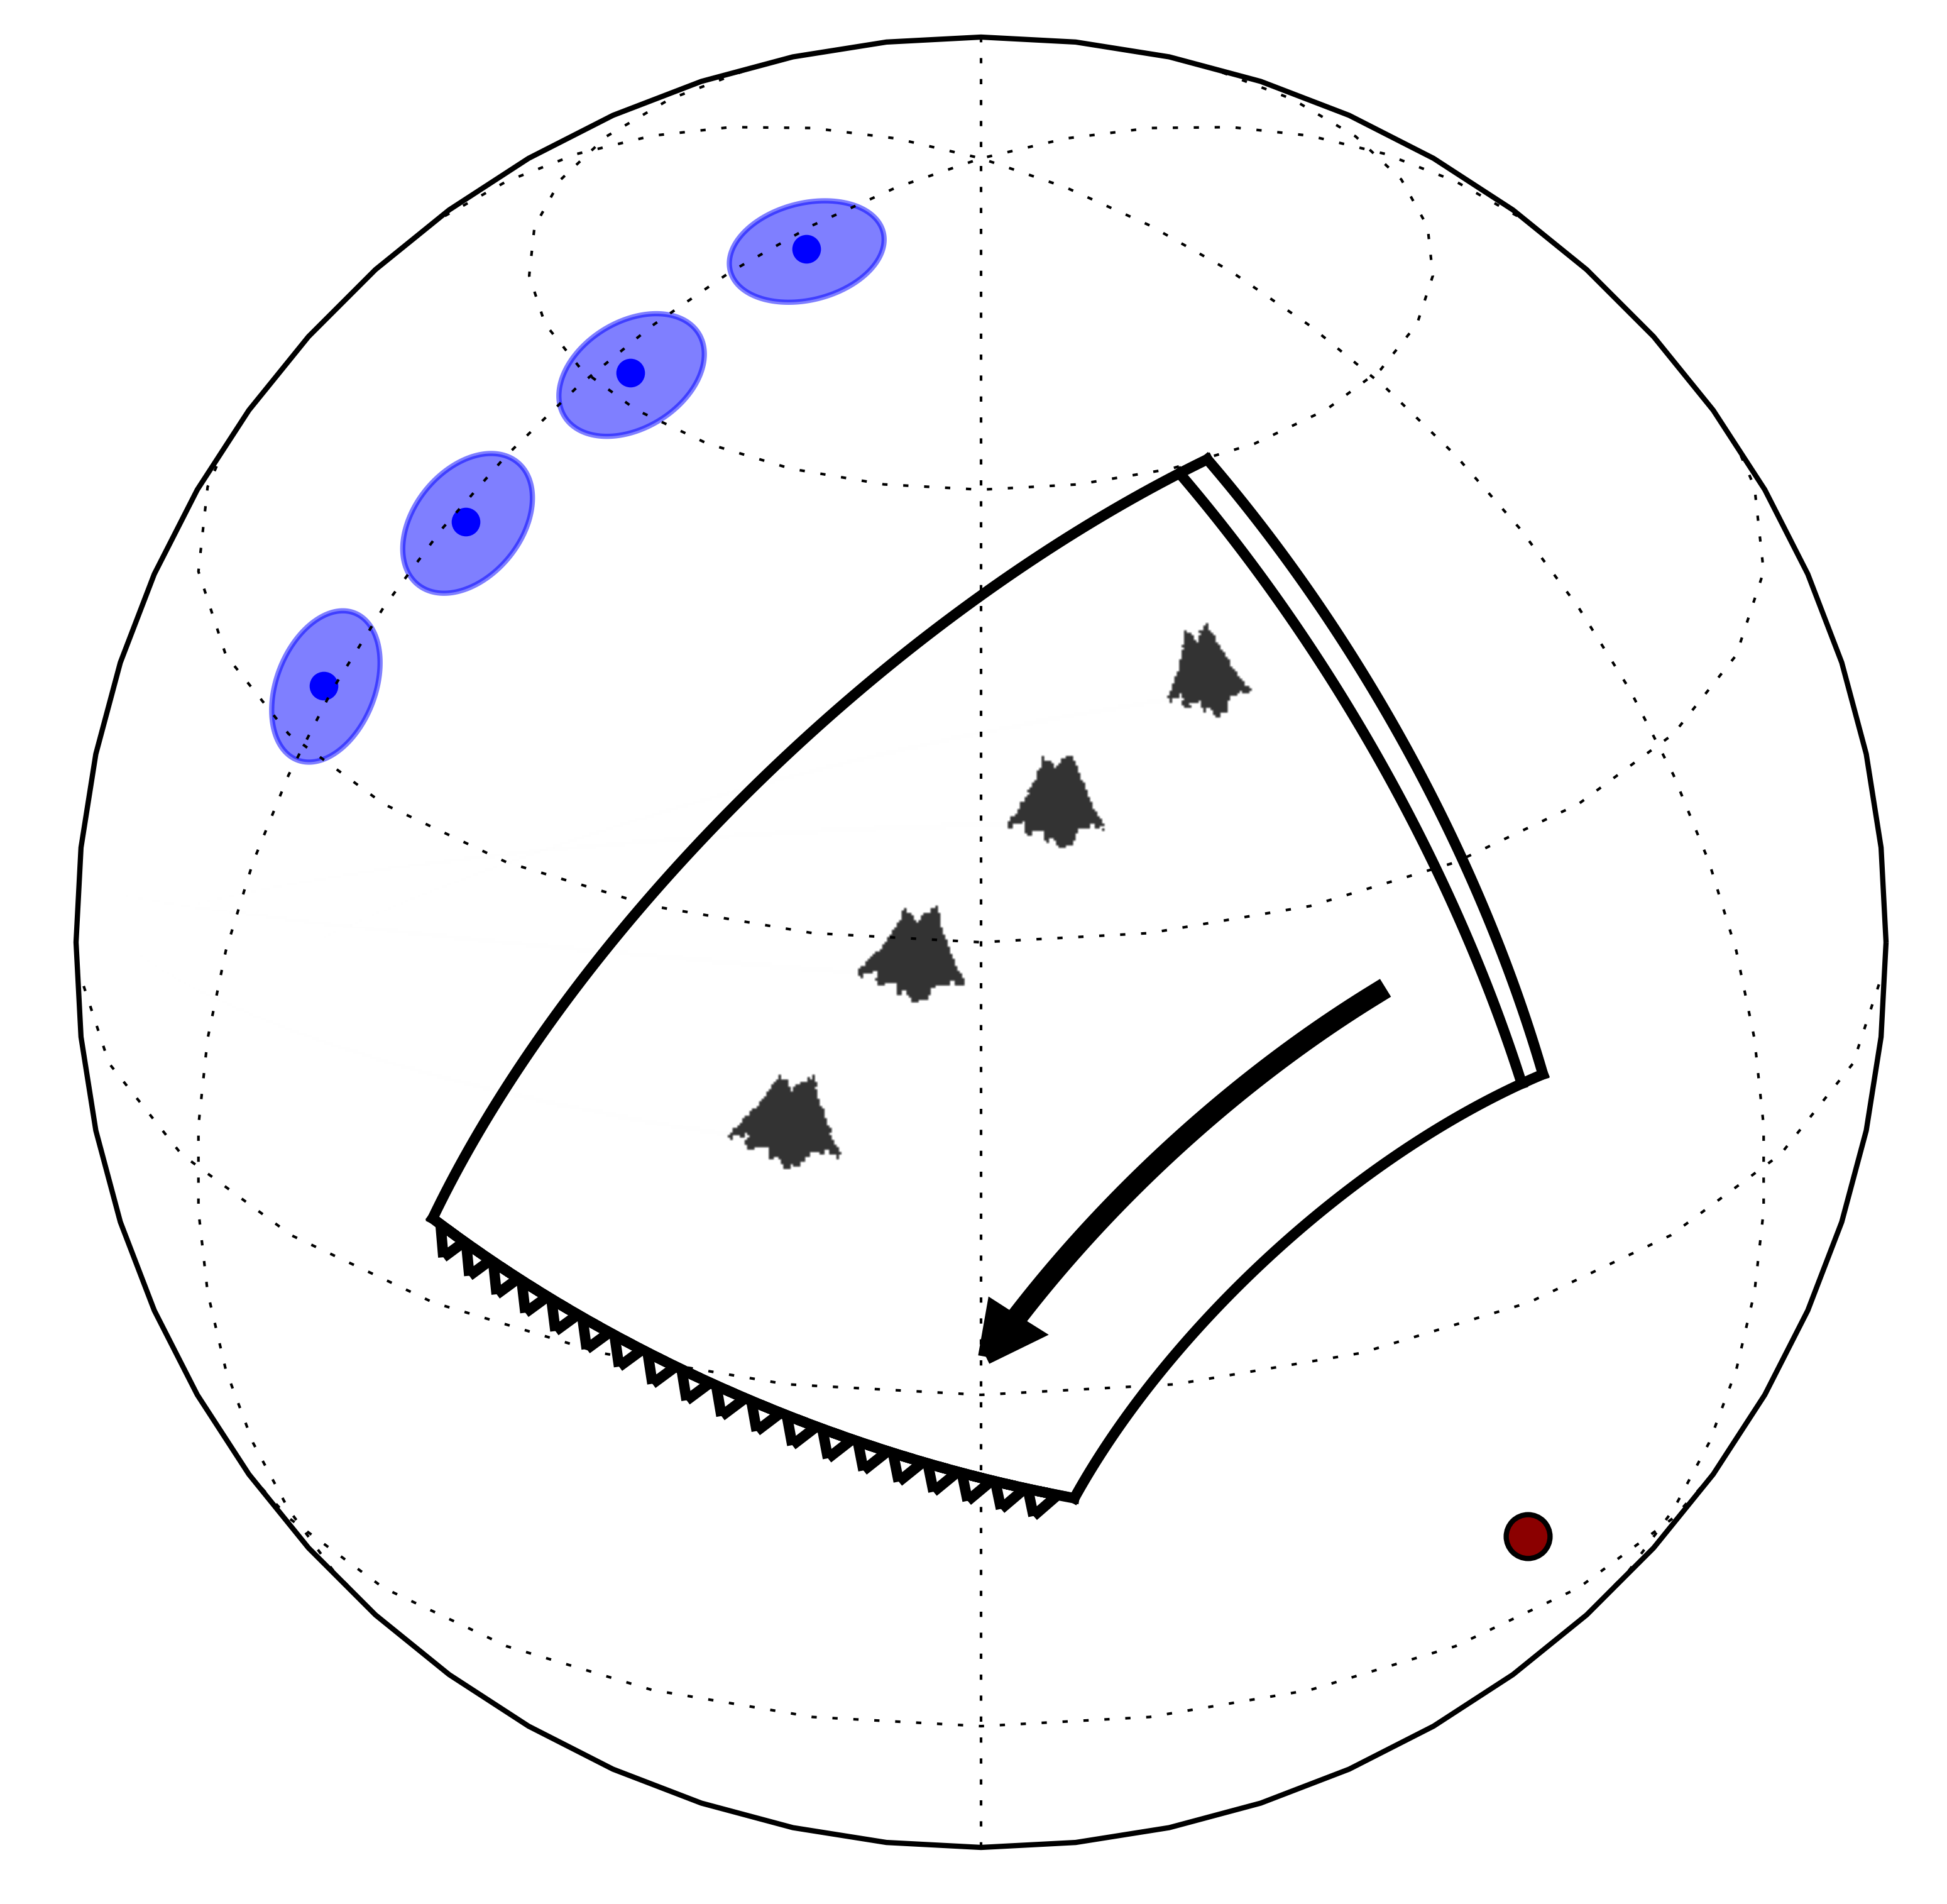
\includegraphics[width=0.5\textwidth]{fig_paleomagnetic_euler_pole.png}
\caption{Conceptual model for a paleomagnetic Euler pole. A finite rotation of a plate around an Euler pole (red circle) results in arcuate oceanic fracture zones and hotspot tracks (cartoon mountain) which describe small circles on the globe. The same finite rotation produces a small/great circle in the APW path, which is illustrated by blue paleomagnetic poles. By fitting a small/great circle to the APWP, we may recover the Euler pole that produced the rotation which is termed the paleomagnetic Euler pole (PEP). Cartoon is adapted from \citet{Gordon1984a}}
\label{fig:pep}
\end{SCfigure}

However, PEP analysis has many of the same deficiencies that spline fits and running means have: it is not easy to compute uncertainties, especially in the presence of unknown ages of poles. Furthermore, one has the additional challenge and related uncertainty of deciding how many PEPs to include for a given sequence of paleomagnetic poles. In this contribution, we develop a Bayesian statistical approach to PEP analysis which attempts to address some of these deficiencies.

\section*{Bayesian inversion}
\subsection*{A general description of inverse problems}

The central question motivating inverse problems is ``How probable is a particular model, given my observations?''. We represent a vector of individual observations by the data vector $\mathbf{d}$, and a model by the vector of model parameters $\mathbf{m}$, so the above question can be expressed as the function $P(\mathbf{m} \vert \mathbf{d})$. Traditional frequentist approaches to an inverse problem often proceed by maximizing the likelihood function, defined by the probability of the data given a particular model \citep[e.g][]{Aster2005a}:
\begin{equation}
\mathcal{L} ( \mathbf{m} \vert \mathbf{d} ) \equiv P( \mathbf{d} \vert \mathbf{m} ).
\label{eq:likelihood}
\end{equation}
The likelihood function replaces something that is difficult to compute (namely, $P(\mathbf{m} \vert \mathbf{d})$)
with something that is less difficult to compute. 
To compute $\mathcal{L}(\mathbf{m}, \mathbf{d})$ we need to have two things: a statistical model for 
uncertainties in the observations $\mathbf{d}$ and a forward model that allows us to compute
predictions. We denote the forward model by $\mathbf{g}$:
\begin{equation}
\mathbf{d}^p = \mathbf{g}(\mathbf{m}),
\label{eq:forward}
\end{equation}
where the superscript ``$p$'' denotes a predicted value.
If each of the observed data $d_i$ are described by Gaussian random variables with standard deviations $\sigma_i$, the likelihood function is given by the product of the individual likelihoods of the observations:
\begin{equation}
\mathcal{L}(\mathbf{d} | \mathbf{m} ) = \displaystyle\prod_i \exp\left({-\frac{(d_i - d_{i}^p)^2}{2 \sigma_i^2}}\right).
\label{eq:example_likelihood}
\end{equation}
The likelihood function $\mathcal{L}$ is maximized by searching over the model parameter space.
If the uncertainties in the observations are Gaussian, then maximizing the likelihood function is
equivalent to the least squares solution \citep{Aster2005a}.

A standard maximum likelihood fit will frequently overfit the observations, resulting in unrealistic solutions. In the context of APWPs, these overfit solutions may pass through every paleomagnetic pole, including less reliable ones, resulting in loopy or jerky paths. In order to address such overfitting, some form of regularization is usually included in the solution of the inverse problem, such as penalizing the magnitude or curvature of the solution. Both the running-mean and the spline under tension approaches to APWPs are a form of regularization on the problem.

\subsection*{Bayesian approach}

The Bayesian approach to inverse problems takes a different strategy from the frequentist one. Rather than finding point estimates of a model fit, it treats the underlying model as a set of random variables with individual probability distributions. The probability distribution of the model $P(\mathbf{m} \vert \mathbf{d})$ given the data  is then found by an application of Bayes theorem \citep[cf.][]{Sivia2006a}:
\begin{equation}
P\left(\mathbf{m} \vert \mathbf{d} \right) = \frac{ P \left(\mathbf{d}\vert \mathbf{m} \right) P \left( \mathbf{m} \right) }{P \left( \mathbf{d}\right).}
\label{eq:bayes}
\end{equation}
It is often unnecessary to calculate the denominator of Equation~\eqref{eq:bayes}, which is a normalization constant, leaving us with
\begin{equation}
P\left(\mathbf{m} \vert \mathbf{d} \right) \propto P \left( \mathbf{d} \vert \mathbf{m} \right) P \left( \mathbf{m} \right).
\label{eq:propbayes}
\end{equation}
The quantity $P(\mathbf{m} \vert \mathbf{d})$ is known as the posterior probability, and it represents our desired knowledge about the distributions of the parameters $\mathbf{m}$. The first factor on the right-hand-side of Equation~\eqref{eq:propbayes} is identical to the likelihood function described above, and the second factor
is known as the prior probability of the model.

The prior probability reflects the state of our knowledge and beliefs of the values of the model parameters prior to the consideration of our data. It also allows us to incorporate constraints that are not otherwise included in the forward model. In contrast with the classical statistical approach of regularization, the Bayesian inverse problem can (in effect) regularize the problem by making
choices of probability distributions that have less probability density in regions with less realistic values \citep[e.g.][]{Minson2013a, Sambridge2013a}.

\subsection*{Markov chain Monte Carlo methods}

It is usually impossible to calculate the posterior probability distribution in Equation~\eqref{eq:bayes} directly \citep{Davidson-Pilon2015a}.  It is much more tractable to generate a Markov chain which, upon convergence, generates samples from the desired posterior \citep{Gelman2013a}. This approach defines a class of methods known as Markov chain Monte Carlo (MCMC) methods.

The literature on MCMC methods is extensive and we do not review it here, but references the interested reader could refer to include \citet{Gelman1996a}, \citet{Sambridge2013a}, and \citet{Davidson-Pilon2015a} for further introduction. A number of high-quality open source software packages for implementing MCMC models exist, including WinBUGS \citep{Lunn2000a}, PyMC3 \citep{Salvatier2016a}, and Stan \citep{Carpenter2017a}. We make extensive use of PyMC3 in this work.

\subsection*{Distributions on a sphere}

In order to proceed with a Bayesian description of the problem, every parameter in the model needs to be described by some statistical distribution that determines the probability that the parameter takes a specific value. Parameters like pole ages can be described by familiar 1D probability distributions (such as uniform or normal distributions), whereas Euler pole locations are described by 2D distributions of directional data on the surface of a sphere. We review several of these distributions here. For a comprehensive discussion of spherical probability distributions, see \citet{Fisher1987b}. Plots of the following distributions (uniform, Fisher and Watson), as well as samples drawn from them, are shown in Figure~\ref{fig:distributions}. 

\subsubsection*{Uniform distribution}
\begin{figure*}
\centering
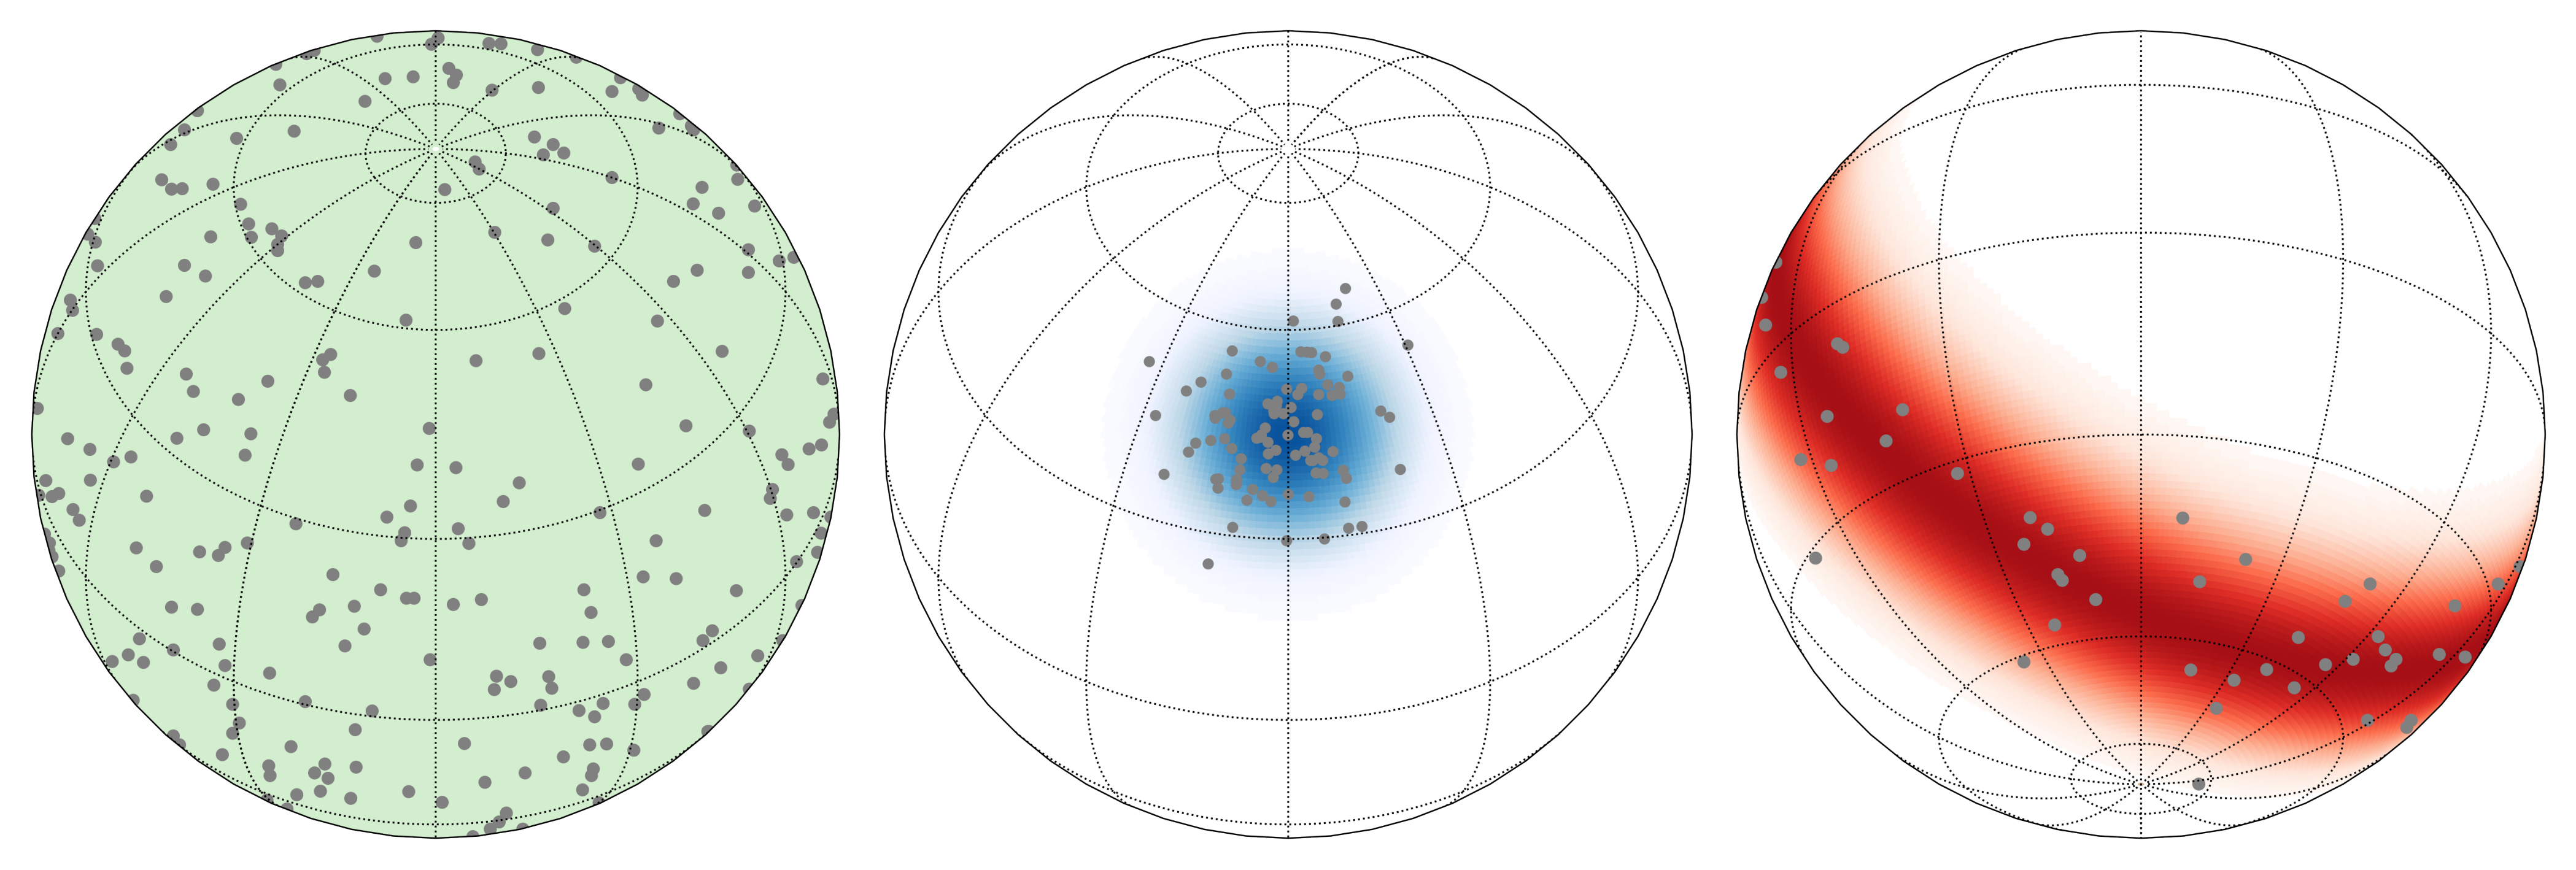
\includegraphics[width=\textwidth]{fig_direction_distributions.png}
\caption[Spherical probability distributions.]{Probability densities for distributions of directional data, as well as samples drawn from them. All distributions are plotted using an orthographic projection. (left panel) Uniform distribution. (middle panel) Fisher distribution. The center of the distribution is at $40^\circ$N, $30^\circ$E, with concentration parameter of $\kappa=50$. (c) Watson girdle distribution. The pole of symmetry is at $30^\circ$N, $30^\circ$E, with a concentration parameter of $\kappa=-25$.}
\label{fig:distributions}
\end{figure*}

The simplest probability distribution on a sphere is the spherical uniform distribution. It has a probability density given by
\begin{equation}
  \rho_U(\phi, \psi) = \frac{1}{4 \pi},
\end{equation}
where $\rho_U$ is the probability density, $\phi$ is the longitude, and $\psi$ is the latitude (we will also refer to the Cartesian unit vector $\hat{\mathbf{x}}$ as a concise representation of $\phi$ and $\psi$). Non-uniform distributions on a sphere reduce to the uniform distribution in some limit (i.e. the Fisher distribution as the precision parameter goes to zero). We will use the uniform distribution when we want to specify an uninformative prior distribution for directional parameters.

\subsubsection*{Fisher distribution}
The Fisher distribution (also called the von Mises-Fisher distribution) is the analogue of a 2D normal distribution on a sphere (Fig. \ref{fig:distributions}). The probability density $\rho_F$ at a point $\hat{\mathbf{x}}$ is given by
\begin{equation}
  \begin{aligned}
  \rho_F(\phi, \psi ; \kappa_F, \hat{\mitbf{\mu}}) 
  &= \frac{1}{C_F} \exp \left( \kappa_F \hat{\mathbf{x}}^T \hat{\mitbf{\mu}} \right) \\
  &= \frac{1}{C_F} \exp \left( \kappa_F \cos \theta \right),
  \end{aligned}
\end{equation}
where $\kappa_F$ is the concentration of the distribution, 
$\hat{\mitbf{\mu}}$ the unit vector for the mean direction of the distribution, and $C_F$ is a normalization coefficient. It can be alternatively parameterized using $\theta$, which is the angle between $\hat{\mathbf{x}}$ and $\hat{\mitbf{\mu}}$.
The normalization factor is given by 
\begin{equation}
  C_F = \frac{\kappa_F}{4 \pi \sinh{\kappa_F}}.
\end{equation}
When $\kappa_F$ goes to zero, the Fisher distribution is equivalent to the spherical uniform distribution.

The uncertainty ellipses for paleomagnetic poles are typically calculated assuming a Fisher distribution of the underlying data, and we will use this distribution to calculate the likelihood function for pole positions in the model.

\subsubsection*{Watson girdle distribution}
Whereas the Fisher distribution concentrates probability density near around a pole on the surface of the sphere, the Watson girdle probability distribution is concentrated in a belt orthogonal to the pole (Fig. \ref{fig:distributions}). It is useful for characterizing planar data, and is given by
\begin{equation}
  \begin{aligned}
  \rho_W(\phi, \psi; \kappa_W, \hat{\mitbf{\mu}}) 
  &= \frac{1}{C_W} \exp \left( \kappa_W (\hat{\mathbf{x}}^T \hat{\mitbf{\mu}})^2 \right) \\
  &= \frac{1}{C_W} \exp \left( \kappa_W \cos^2 \theta \right),
  \end{aligned}
\label{eq:watson}
\end{equation}
where $\kappa_W$ is the concentration of the girdle, $C_W$ is a normalization coefficient, and the other parameters are identical to those in the Fisher distribution. The Watson distribution is girdle-shaped only when $\kappa_W$ is a negative number, which is the only case we consider here.

The normalization factor is given by
\begin{equation}
  C_W = \left[ {}_1 F_1 \left( \frac{1}{2}, \frac{3}{2}, \kappa_W \right) \right]^{-1},
\end{equation}
where ${}_1 F_1()$ is Kummer's confluent hypergeometric function, which is available in most software libraries of special mathematical functions. As with the Fisher distribution, when $\kappa_W$ goes to zero,  the Watson distribution is equivalent to the spherical uniform distribution.

\section*{A model for PEP inversion}
\label{sec:model}
\subsection*{Forward model}
\label{sec:forward_model}
A forward model describes how we generate predicted observations, given a set of model parameters (Equation~\eqref{eq:forward}). The forward model for PEP analysis in this study is essentially unchanged from that of \citet{Gordon1984a}. We describe plate motions (and hence paleomagnetic pole motions) with a series of Euler poles. Each Euler pole has three parameters: a latitude, a longitude, and a rotation rate.

We also must specify the ages where we switch from one Euler pole to the next (the cusps, or ``hairpins'' of \citet{Irving1972a}). In the context of parameter inversion, these ages are often known as ``changepoints.''

Finally, we need a starting position on the globe, which, in practice, can be sampled from the Fisher distribution of the oldest paleomagnetic pole in the data set. The starting point contributes two parameters (a latitude and a longitude).

Therefore, a model with $n_e$ Euler rotations will have $3 n_e$ parameters for the poles, $(n_e-1)$ parameters for the changepoints, and 2 parameters for the starting location. The number parameters for which we are inverting is then given by
\begin{equation}
\begin{aligned}
N &= 3 n_e + (n_e -1) + 2 \\
 &= 4 n_e + 1.
\end{aligned}
\label{eq:n_parameters}
\end{equation}

For each Euler pole, $\mitbf{\omega}_i$ the velocity $\mathbf{v}$ of a point $\mathbf{p}$ on the surface of the globe is given by
\begin{equation}
\mathbf{v} = \mitbf{\omega}_i \times \mathbf{p}.
\label{eq:rigid_rotation}
\end{equation}
Finite rotations can be performed by constructing Euler angle rotation matrices \citep[cf.][]{Goldstein1965a}.  We generate synthetic paleomagnetic pole positions from the forward model by stringing together finite rotations through the stage poles until the age of the paleomagnetic pole is reached. These positions can then be compared to the actual paleomagnetic poles in our dataset.

\subsection*{Choice of prior distributions}
\label{sec:priors}

Bayesian analysis requires us to specify prior probability distributions for each of the model parameters in the inverse problem. These distributions reflect our state of knowledge about the values of the parameters before we begin, and allow us the option of incorporating information otherwise not captured by the model. To avoid biasing the results of the model towards a specific posterior distribution, we usually try to choose prior distributions that are as uninformative as possible. Depending upon the context, and the type of parameter, that choice may vary. The central parameters in the paleomagnetic Euler pole problem are the Euler pole positions, the Euler pole magnitudes, the changepoints, the starting point, and the paleomagnetic pole ages, which we treat in turn. We use the notation $x \sim y$ to indicate that the parameter $x$ is drawn from distribution $y$.

\textbf{Euler pole directions:} 
The first parameter we consider is the position of the Euler poles, which should be drawn from a spherical probability distribution. The least informative prior distribution for the i'th Euler pole is the uniform spherical distribution:
\begin{equation}
\hat{\mitbf{\omega}}_i \sim \rho_U.
\end{equation}
essentially allowing the Euler pole to be anywhere on the globe with equal probability.

An interesting alternative choice is to inform our prior distribution for Euler pole position based on current plate motions. It has long been observed that, to first order, plate motions are well explained by slab-pull torques acting along subduction zones, and to a lesser extent, ridge push and mantle traction effects \citep{Forsyth1975a, Gordon1978a, Richardson1992a}. 

We can ask the question of whether the Euler pole for a given plate is more likely to be on top of the plate (corresponding to a spinning motion for that plate) or far away from that plate (corresponding to motion across the surface of Earth). Given that tectonic plates can broadly be considered to be the surface expression of mantle convection, we can hypothesize that the second possibility is more likely because a spinning plate has no divergence (i.e., spreading centers and subduction zones, \citep{Forte1987a, Gable1991a}).  Without divergence the plate motion does not contribute to convection.

To test this hypothesis, we generated position samples on the surface of Earth and computed the angular distance between that point and the Euler pole for the plate in which that point resides. We used the NNR-MORVEL56 model for current plate motions \cite{Argus2011a} and restricted our analysis to the fourteen largest plates. We then fit those angular distance samples to a Watson girdle distribution (Equation~\eqref{eq:watson}),  inverting for the concentration parameter $\kappa_W$. If an Euler pole position has no preference for being a particular angular distance from a point on a plate, then $\kappa_W$ should be close to zero, corresponding to a uniform distribution. We find that the distribution is best fit with $\kappa_W \approx -0.8$, which corresponds to the Euler pole probability density being roughly twice as large $90^\circ$ away from a given point than on top of the point (Fig.~\ref{fig:euler_pole_prior}).

\textbf{Euler pole magnitudes:} 
The magnitude of each Euler pole is a positive number, specifying the rotation rate of that pole (negative rotations can be accommodated by flipping an Euler pole to the antipode). There are several possibilities for the prior distribution for the rates. In order to not bias the inversion towards a particular rate, we can choose a uniform prior distribution with large support:
\begin{equation}
\vert \mitbf{\omega}_i \vert \sim U(0, 4),
\end{equation}
where $U(\cdot, \cdot)$ is a uniform distribution between two values, and is specified  in degrees per Myr. Typical rotation rates for present day plate motions are under $1^\circ$/Myr \citep{Argus2011a}, which corresponds to rates of about 11 cm/yr at a position $90^\circ$ from the Euler pole.

Another option is to choose a weakly informative prior distribution for the Euler pole magnitudes informed by recent plate motions (similar to the Watson girdle prior distribution for Euler pole position). \citet{Zahirovic2015a} found, based on analysis of Cenozoic and Mesozoic plate reconstructions, that plate speeds much higher than 15 cm/yr were unlikely to be sustained. A reasonable choice of distribution for strictly positive numbers is the exponential distribution, given by
\begin{equation}
\rho_E(\vert \mitbf{\omega}_i \vert) = \lambda \exp(-\lambda \vert \mitbf{\omega}_i \vert),
\end{equation}
which has higher probability density at lower values, and falls off exponentially. We sampled the current plate rates on Earth's surface according to NNR-MORVEL56 and fit those to an exponential distribution. The best fitting scale parameter $\lambda$ for current plate rates is $\lambda\approx2.5$ (Fig.~\ref{fig:euler_pole_prior}). Making this choice of prior distribution for Euler pole rotation rates can be seen as a form of regularization on plate speeds.

\begin{figure*}
\centering
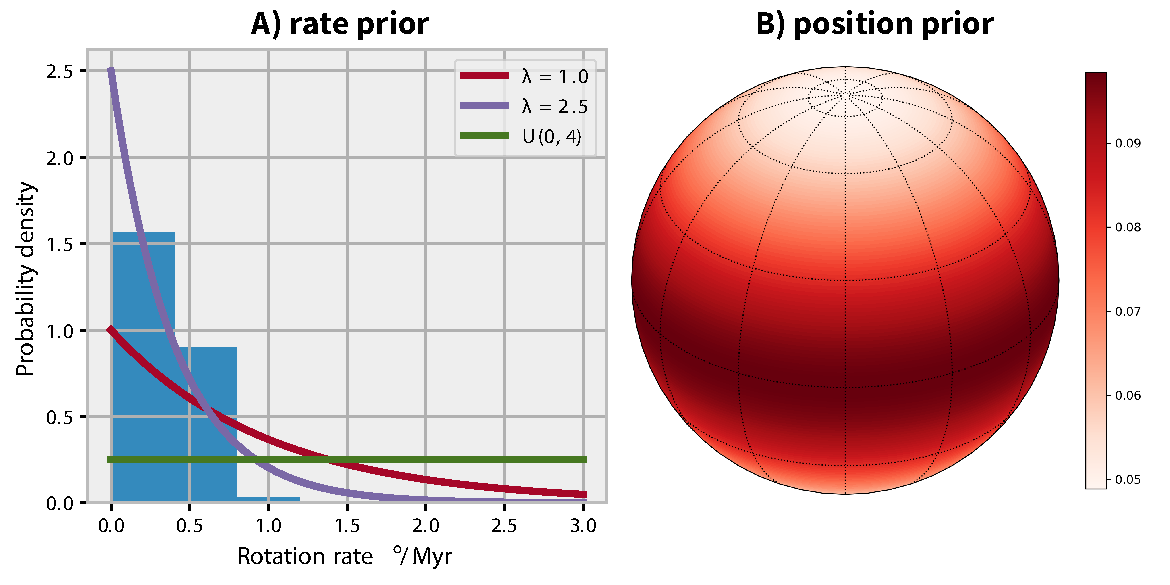
\includegraphics[width=0.9\textwidth]{fig_euler_pole_prior.pdf}
\caption[Informative prior distributions for Euler poles]{Informative prior distributions for Euler poles. (a) Prior probabilities for rotation rates. The histogram is the angular rotation rate from one thousand samples from the surface of Earth, using the NNR-MORVEL56 model. A fit to this sample set with an exponential distribution yields a scale parameter of $\lambda \approx 2.5$. We also show the distribution for $\lambda = 1.0$, which imposes less regularization on the rate as a less restrictive prior distribution, and a uniform $U(0,4)$ distribution between 0 and 4\textdegree/Myr, which specifies no preference for slower speeds if set as the prior probability. (b) Prior probability density for the position of the Euler poles, with the north pole as the site latitude and longitude.  We again sampled one thousand points on Earth's surface, calculating the angular distance between that point and the Euler pole for its plate.  If we model the probability distribution as being drawn from a Watson distribution, these angular distances correspond to colatitudes, where the pole is the sampled point.  Fitting the resulting angular distribution to a Watson girdle distribution finds $\kappa_W \approx -0.8$. Since the Watson distribution is rotationally symmetric, longitudes do not contribute to the fit. For $\kappa_W \approx -0.8$ the probability density is roughly twice as large at the equator (90\textdegree from a plate) as at the pole (on top of the plate).}
\label{fig:euler_pole_prior}
\end{figure*}

\textbf{Changepoints:} 
Changepoints occur sequentially between the oldest (at age $a_\mathrm{max}$) and youngest (at age $a_\mathrm{min}$) paleomagnetic poles. We choose a uniform distribution as a prior for these changepoints:
\begin{equation}
c_i \sim U( a_\mathrm{min}, a_\mathrm{max}),
\end{equation}
where $c_i$ is the i'th changepoint.

\textbf{Starting position:}
Finally, the starting position $\hat{\mathbf{x}}_\mathrm{start}$ for the set of Euler pole rotations needs a prior distribution. We could choose another uniform distribution, but a more reasonable choice is to start near the oldest paleomagnetic pole in the dataset. We therefore choose the Fisher distribution of the oldest paleomagnetic pole as a reasonable prior distribution for a start point:
\begin{equation}
\hat{\mathbf{x}}_\mathrm{start} \sim \rho_F(\kappa_{F0}, \hat{\mitbf{\mu_0}}),
\end{equation}
where $\kappa_{F0}$ and $\hat{\mitbf{\mu}}_0$ are the concentration parameter and mean direction of the oldest paleomagnetic pole in the dataset.

\textbf{Pole ages:}
One of the major advantages of Bayesian analysis is the ability to naturally incorporate uncertainties in as many parameters as needed. Previous approaches to modeling APWPs have the drawback that they do not easily account for uncertainties in the age of paleomagnetic poles. In our approach, we can include age uncertainty by including the age of the poles and associated uncertainty as parameters in our model.

There are many different ways to constrain the ages of the geologic units from which we obtain paleomagnetic poles, including radiometric dating, biostratigraphy, magnetostratigraphy, cross-cutting relationships, and stratigraphic relationships. Here we concentrate on poles that are either interpreted to be the age of a single radiometric date or are interpreted to be bracketed stratigraphically between two dates (derived radiometrically or by using other age control such as biostratigraphy). If a geologic unit has been radiometrically dated, we can model the age of the j'th paleomagnetic pole $a_j$ as a normal distribution with mean $\mu_j$ and standard deviation $\sigma_j$:
\begin{equation}
a_j \sim N(\mu_j, \sigma_j),
\end{equation}
where $N(.,.)$ denotes a normal distribution.

Frequently, however, the geologic unit from which we obtain a paleomagnetic pole is not well dated, but its age can be constrained to lie between those of well-dated units stratigraphically above and below it or dates obtained by cross-cutting relationships. In these cases, a uniform distribution between those ages is a reasonable choice for the prior distribution:
\begin{equation}
a_j \sim U(a_\mathrm{young}, a_\mathrm{old}),
\end{equation}
where $a_\mathrm{young}$ and $a_\mathrm{old}$ are the ages of the lower and upper age constraints, respectively.

To summarize our choices for prior distributions:
\begin{itemize}
\item Euler pole positions: spherical uniform distribution, or a Watson girdle distribution with $\kappa_W \approx -0.8$.
\item Euler pole magnitudes: Uniform distribution between 0$^\circ$ and 4$^\circ$/Myr, or an exponential distribution with $\lambda \approx 2.5$.
\item Changepoints: uniform distribution between $a_\mathrm{min}$ and $a_\mathrm{max}$.
\item Paleomagnetic pole ages: normal or uniform distribution, depending on the type of age control for the geologic unit from which the pole was obtained.
\end{itemize}

\subsection*{Likelihood}
\label{sec:likelihood}
In addition to the choice of prior distributions, we need a statistical description of the observations. This description will allow us to calculate the likelihood function, which, when combined with the prior distributions, allows us to evaluate Bayes' theorem (Equation~\eqref{eq:propbayes}).

In the case of APWPs, our observations are paleomagnetic poles. The most common statistical distribution for describing paleomagnetic poles is the Fisher distribution (although other distributions are sometimes used, such as the Kent or Bingham distributions, c.f. \citet{Tauxe2010a}). Given the set of model parameters $\mathbf{m}$ and the forward model $\mathbf{g}(\mathbf{m})$, described above, we can calculate the predicted paleomagnetic pole unit vectors $\hat{\mathbf{x}}_i^p$. For a set of $n$ paleomagnetic poles, the likelihood is then given by the product of the probabilities of each observation:
\begin{equation}
P(\mathbf{d} \vert \mathbf{m}) = \displaystyle\prod_{i=1}^n \frac{1}{C_{F,i}} \exp \left( \kappa_{F,i} \hat{\mathbf{x}}_{i}^{pT} \hat{\mitbf{\mu}}_i \right).
\label{eq:model_likelihood}
\end{equation}

\section*{Example inversions}
\label{sec:example_inversion}

Before proceeding with inversions for paleomagnetic Euler poles using real paleomagnetic data, it is useful to consider a few examples of inversions for synthetic datasets. We have specified the forward model described above using the package PyMC3 \citep{Salvatier2016a} which enables us to perform the inversion. Within PyMC3, we are able to specify custom probability distributions enabling the directional data distributions illustrated in Figure \ref{fig:distributions} to be implemented. The Markov chain Monte Carlo (MCMC) analysis uses the Metropolis–Hastings algorithm for sampling. Our code for the inversions has an open-source GPL license and may be found at \url{https://github.com/Swanson-Hysell-Group/Bayesian_PEP_inversion}. \textit{we will also archive the repository on Zenodo at the time of proofs following any revisions}

%In most cases shown here, we generate $10^6$ samples and discard the first 20\% to avoid potential bias in the posterior due to a poor starting point. 

% In all of the inversions we show here, we choose $\kappa_W=0$ for the Watson concentration parameter in the Euler pole direction prior distribution (that is, equivalent to a uniform distribution on a sphere), and $\lambda=2.5$ for the scale parameter in the Euler pole magnitude prior distribution.

\subsection*{One Euler rotation}
\label{sec:one_stage_pole}
We begin by trying to recover the Euler pole for a single rotation. We generate an idealized synthetic APW track of four poles by starting from a pole at $19^\circ$ N, $24^\circ$ E, and rotating around an Euler pole at $00^\circ$ N, $000^\circ$ E for 100 Myr at a rate of $1^\circ$/Myr. We produce paleomagnetic poles at 100 Ma, 75 Ma, 50 Ma, and 25 Ma, and prescribe $A_{95}$ of $4^\circ$ to each pole (where $A_{95}$ indicates the 95\% angular confidence interval for the pole position).

The results of the inversion are shown in Figure~\ref{fig:synthetic_pep}. The Bayesian approach successfully recovers a posterior probability distribution for the position of the Euler pole that includes the start pole, as well as a rate that is centered near the true value of $1^\circ$/Myr (Fig.~\ref{fig:synthetic_pep}). The posterior distribution for the rate has a highest posterior density (HPD) credible interval at 95\% (which we abbreviate from here as a 95\% credible interval) between $0.8^\circ$/Myr and $1.2^\circ$/Myr, reflecting the resolving power of the inversion for data with the given uncertainties.

\begin{figure*}
\centering
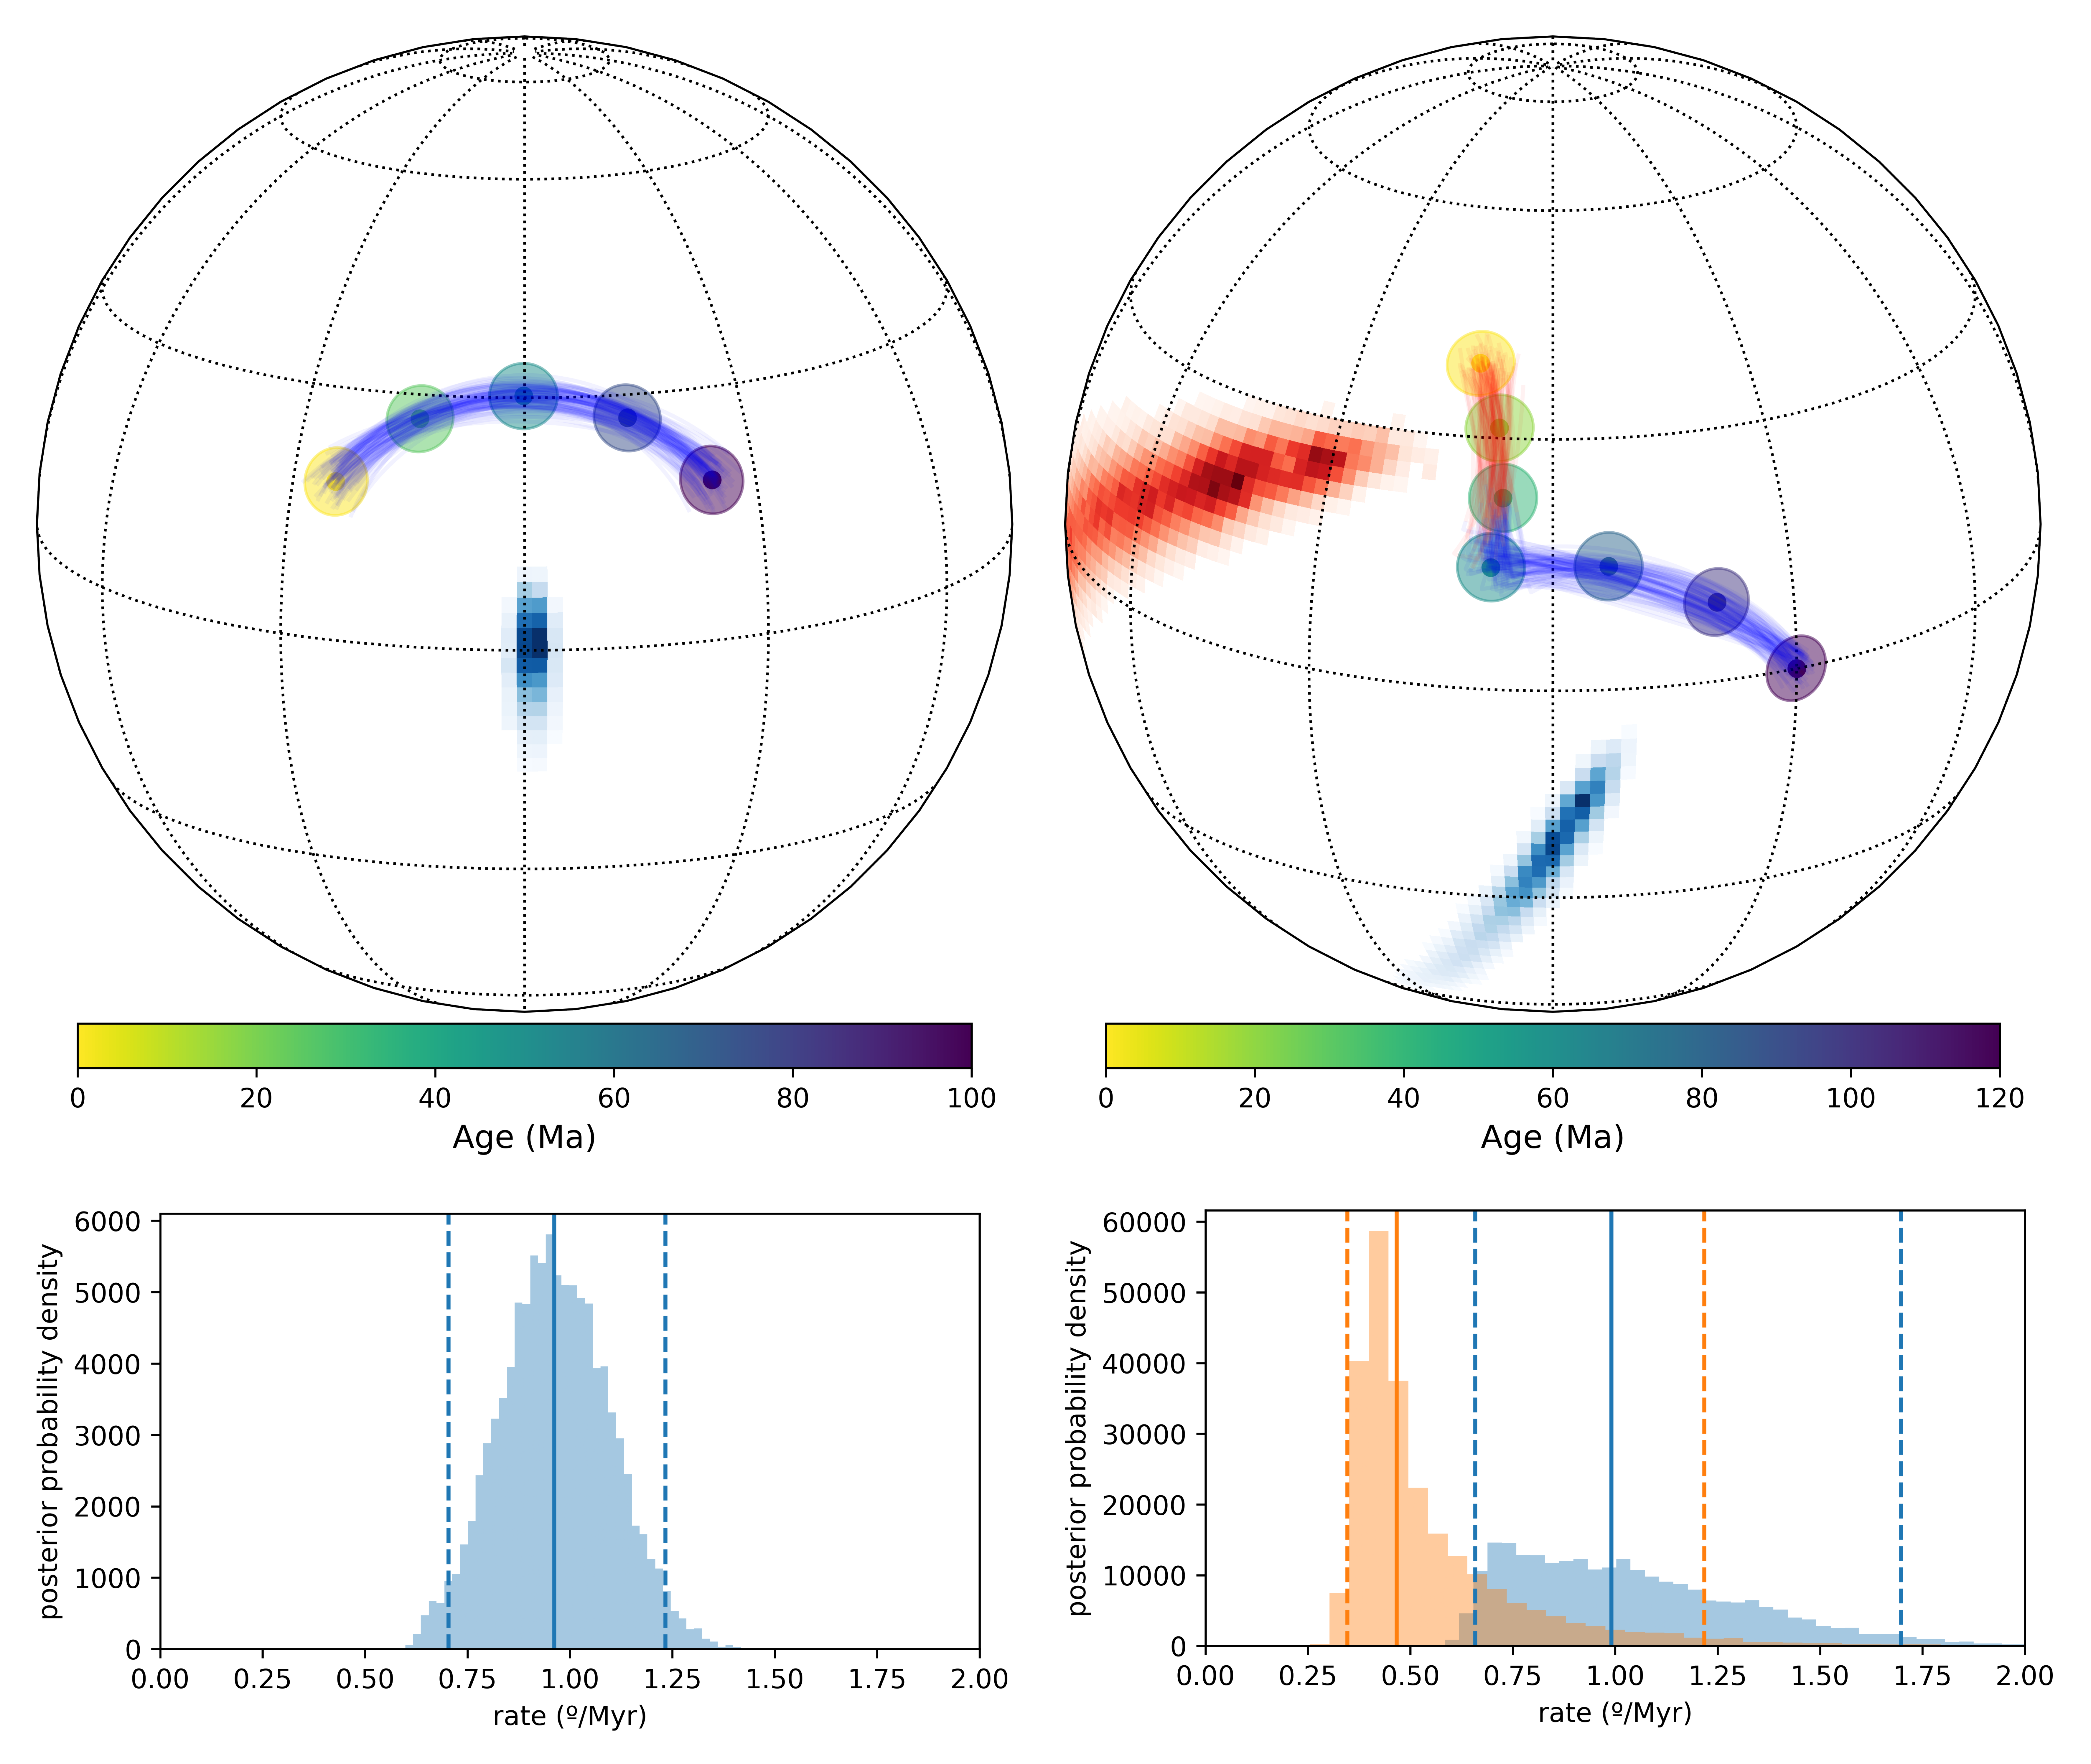
\includegraphics[width=0.9\textwidth]{fig_synthetic_pep.png}
\caption{Inversion for Euler poles from synthetic data. (upper left) Five paleomagnetic poles are generated during a net $100^\circ$ rotation about an Euler pole at $00^\circ$N, $000^\circ$E over 100 Myr, for a rotation rate of $1^\circ$/Myr. The blue distribution is the probability density of Euler pole positions recovered by MCMC inversion, and the blue arcs are a sampling of 100 synthetic APWPs generated by the inversion. (lower left) Posterior probability density for the rotation rate of the Euler pole recovered by the inversion. The solid line shows the median of the distribution ($0.96^\circ$/Myr), and the dashed lines show the 95\% credible interval ($0.70^\circ-1.23^\circ$/Myr). (upper right) Paleomagnetic poles generated using two distinct Euler poles. The first Euler pole is located at $10^\circ$S, $000^\circ$E, and rotates at $1.5^\circ$/Myr for 60 Myr. The second Euler pole is located at $10^\circ$N, $300^\circ$E, and rotates at a speed of $0.75^\circ$/Myr for 60 Myr. The blue and red distributions show the posterior estimate location of the first and second Euler poles (respectively) recovered by the MCMC inversion. The blue and red arcs are a sampling of 100 synthetic APWPs generated by the inversion. (lower right) Posterior probability density for the rotation rates of the Euler poles recovered by the inversion. The solid lines show the median values of the distributions ($\sim 1.45^\circ$/Myr and 0.76$^\circ$/Myr for Euler rotation 1 and 2), and the dashed lines show the 95\% credible intervals.}
\label{fig:synthetic_pep}
\end{figure*}


\subsection*{Two Euler rotations}
\label{sec:two_stage_poles}
We next consider an inversion for an APW track with two stage poles. Unlike the previous example that inverted for a single Euler pole, this inversion also requires a changepoint. We generate nine idealized paleomagnetic poles with $A_{95}$ of $4^\circ$ from a starting point at $5^\circ$S, $030^\circ$E. The first rotation is around an Euler pole at $10^\circ$S, $000^\circ$E, and rotates at $1.5^\circ$/Myr for 60 Myr. The second rotation is around an Euler pole at $10^\circ$N, $300^\circ$E, rotates at a rate of $0.75^\circ$/Myr for the same amount of time. The synthetic poles associated with this two stage model are shown in Figure~\ref{fig:synthetic_pep}. 

The inversion successfully recovers the Euler pole rotation rates with posterior distributions centered near the true values. The inverted Euler pole positions for the first stage pole (Figure~\ref{fig:synthetic_pep} blue distributions) are centered near the true location (Figure~\ref{fig:synthetic_pep} blue star) and the inverted second Euler pole positions encompass the true location as well. In comparison with the first stage Euler pole, the more spatial uncertainties associated with the second Euler pole reflects that paleomagnetic poles constrain the Euler pole to lie along a great circle perpendicular to the trend of the APW small circle but the location of the Euler pole along the great circle can be difficult to constrain when the $A_{95}$ uncertainties are large relative to the arc distance between paleomagnetic poles. Nevertheless, the posterior distributions successfully recovers the change in Euler rotation rates and the changepoint is centered near 60 Ma. This example demonstrates the inversion can resolve APW paths with more than one stage poles and provides posterior distributions that informs the timing of Euler rotation change without any informed prior knowledge (Figure~\ref{fig:synthetic_pep}).

\subsection*{Incorporating age uncertainty}
\label{sec:age_uncertainty}
A major benefit of the Bayesian approach to inverse problems is its generality. As long as some effect can be described statistically and incorporated into our forward model, we can include it in the inverse problem.

In this case, we include uncertainties in the ages of the paleomagnetic poles. We use the a similar test case as in the one Euler pole inversion with the ages of synthetic poles being adjusted to span from 140 Ma to 40 Ma, but assign uncertain prior distributions to the ages of the poles. For the first and last poles we assume they are radiometrically dated with standard deviations of 5 Myr. However, we assume that the middle three poles have no age control, except that their
respective rock units lie stratigraphically between the first and last poles. We thus assign Gaussian prior distributions to the first and last poles and uniform prior distributions
to the middle three.

For real data, adding uncertainties to the ages of the poles enables us to properly represent our knowledge of the constraints on the APWP. Additionally, these uncertainties enable data to constrain the location of the path without providing an overly tight constraint on the timing.
Figure~\ref{fig:age_uncertainty_samples} shows the prior and posterior distributions for the ages of the poles. We can see from the posterior distribution that the inversion successfully places the ages of the middle three poles at $\sim115$ Ma, $\sim90$ Ma,  and $\sim65$ Ma. However, the 95\% credible intervals on these age estimates are relatively wide. The posterior distributions for the Euler pole position and magnitude which we recover from this inversion are very similar to those in Figure~\ref{fig:synthetic_pep}.

\begin{figure*}
\centering
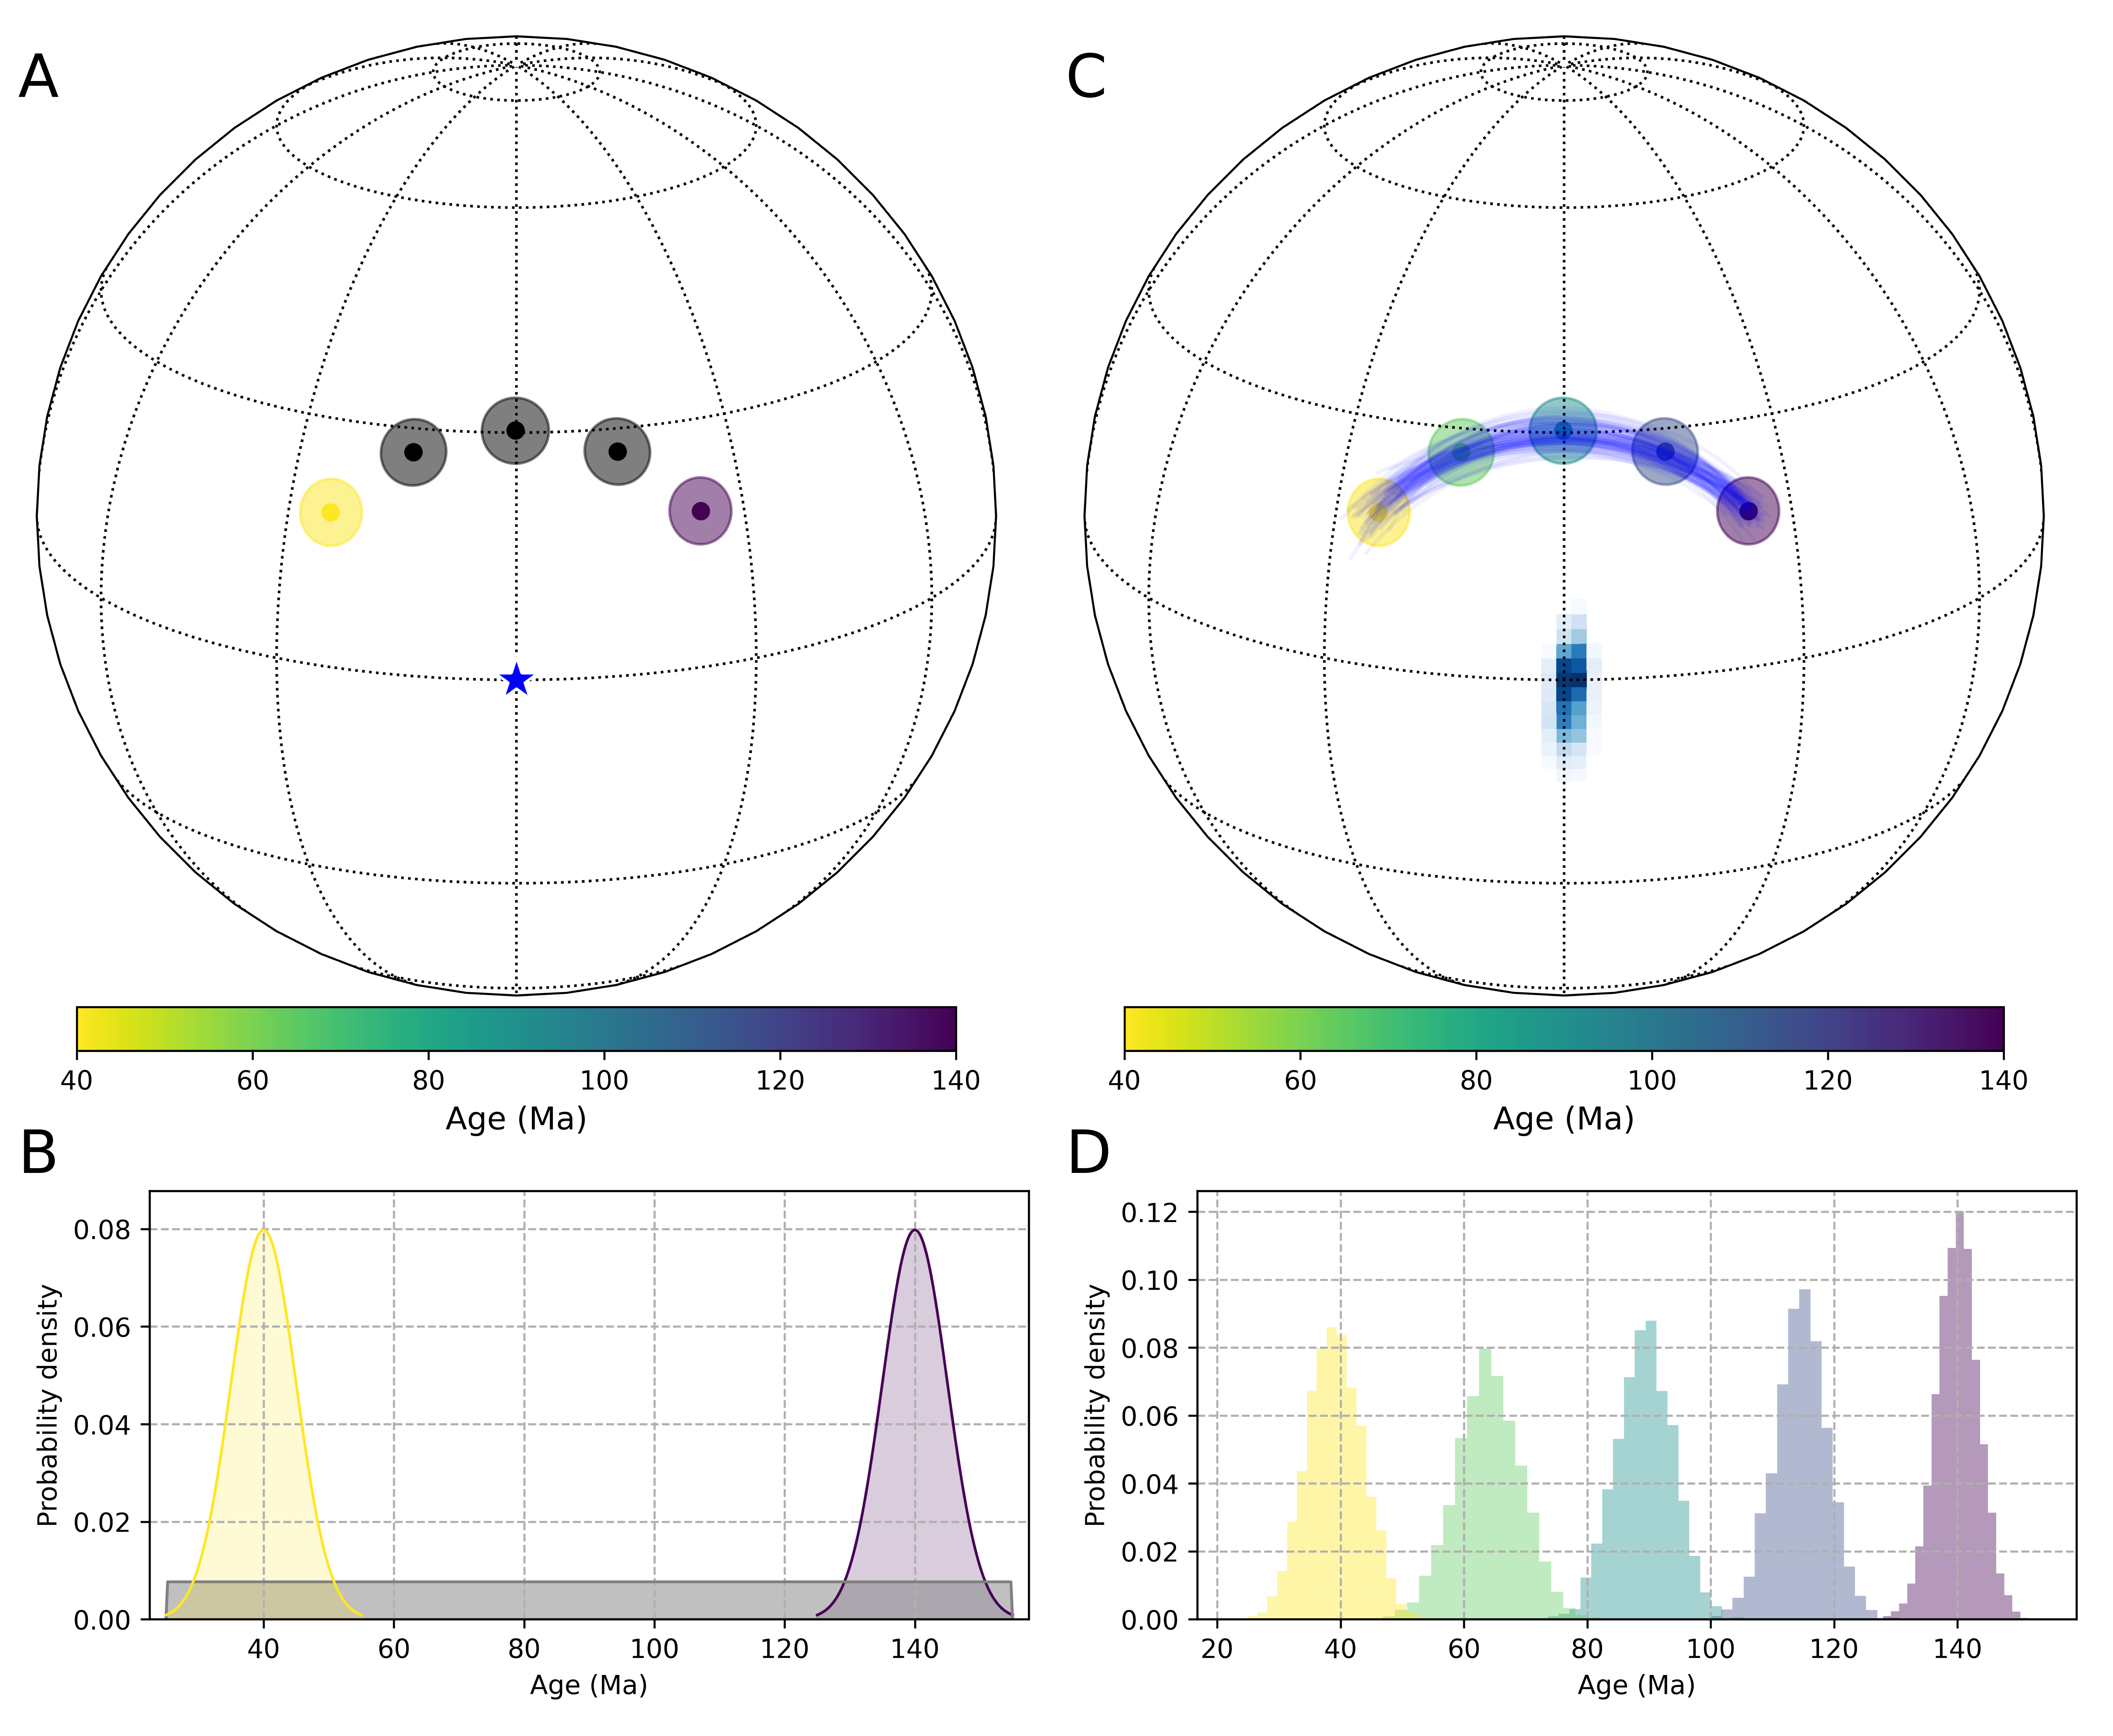
\includegraphics[width=0.9\textwidth]{fig_inversion_with_age_uncertainties.png}
\caption[Probability distributions for ages of the paleomagnetic poles in the one-Euler pole inversion test.]{Probability distributions for the ages of the paleomagnetic poles in the one-Euler pole inversion test. Left panels: prior knowledge about paleomagnetic poles positions and ages. We presume the first and last poles to be radiometrically dated with one-sigma uncertainties of 5 Myr, and are assigned Gaussian prior distributions. The middle two poles are undated, and are only stratigraphically constrained to be between the first and last poles. Right panel: posterior distributions after $10^5$ MCMC samples. The distributions of the first and last samples are largely unchanged, but the distributions for the middle three poles are centered on their true values of 115 Ma , 90 Ma, and 65 Ma. Importantly, the middle poles help to constrain the location of the Euler pole, but the wide prior distributions on their ages do little to constrain the rotation rates.}
\label{fig:age_uncertainty_samples}
\end{figure*}

\subsection*{Reporting the apparent polar wander path}
\label{sec:age_uncertainty}
A difficulty with the Bayesian approach is that the credible interval of Euler pole solutions are not easy to report as they do not neatly correspond to a parametric statistical distribution. We visualize the solutions with spatial histograms for the Euler pole positions and by showing example inverted paths. A typical product that one is seeking with such an inversion is an apparent polar wander path reported as interpreted pole position at given intervals. An approach that can be taken is to calculate a number of predicted pole positions at a given time implied by inverted Euler pole models and then to calculate the Fisher mean of these inverted pole positions. This approach provides the mean pole position on the apparent polar wander path. We also wish to report the uncertainty on that estimated position. The spread in the position of these inverted pole positions has real meaning related to the certainty of the position within the inversion that corresponds both to the best-fit in space through the poles and that in time which affects the rate of the rotation about the Euler pole. The spread in pole positions can be approximated as a Fisher distribution from which the angle from the mean that contains 95$\%$ of the solutions ($\theta_{95}$) can be calculated:
\begin{equation}
\theta_{95}=\frac{140^{\circ}}{\sqrt{\kappa}}
\label{eq:angular_deviation}
\end{equation}
This angle is equivalent to a 2$\sigma$ uncertainty in Gaussian statistics. Implied pole positions from these inversions are more tightly clustered than the inverted Euler pole positions themselves and typically are consistent with being drawn from a Fisher distribution such that reporting the 95$\%$ confidence of angular deviation is appropriate.

\section*{Application to the Keweenawan track}
\label{sec:keweenawan}

An impetus for the development of this Bayesian paleomagnetic Euler pole inversion method was to constrain the absolute rates of plate motion associated with the ca. 1109 to 1070 Ma Keweenawan Track of paleomagnetic poles \citep{Swanson-Hysell2009a, Swanson-Hysell2019a}. These poles are associated with the rapid motion of Laurentia towards the equator leading up to the Grenvillian orogeny and the assembly of the supercontinent Rodinia \citep{Swanson-Hysell2021a}. While previous approaches had established estimates for the rate of latitudinal motion associated with the Keweenawan Track \citep{Davis1997a, Swanson-Hysell2014b}, we implemented this method in \citet{Swanson-Hysell2019a} in order to constrain absolute rates (without providing details on the methodology that are elucidated in the present contribution). In addition to our goals of constraining absolute rates, this approach was particularly appropriate for the Keweenawan Track as it includes poles with quite disparate precision on their age constraints as some are constrained tightly by high-precision U-Pb dates \citep[e.g.][]{Fairchild2017a} while others have looser radiometric constraints. A technical note related to the analysis in \citet{Swanson-Hysell2019a} is that it used a version of the code written in PyMC2 (\citealp{Patil2010a}; \url{https://github.com/ian-r-rose/mcplates}). The PyMC project has migrated to PyMC3 which is a total rewrite of the code \citep{Salvatier2016a} and necessitated our code to refactored into its present version (\url{https://github.com/Swanson-Hysell-Group/Bayesian_PEP_inversion}). 

\begin{figure*}
\centering
\includegraphics[width=0.7\textwidth]{fig_Keweenawan_Track.pdf}
\caption{A) Bayesian PEP inversion of the Keweenawan Track using three different combinations of Euler poles. The Euler pole locations and representative resulting tracks along with modeled pole positions are shown with the paleomagnetic poles. The distribution of plate speed associated with each inverted Euler pole is shown in the histograms with the 95$\%$ credible interval indicated with dashed lines. B) The upper plot illustrates the prior probability distributions for the ages of the paleomagnetic poles used in the inversion. Poles with radiometric ages are assigned Gaussian distributions while those with stratigraphic age control are assigned uniform distributions between bracketing ages. The posterior probability of poles ages resulting from the one plate tectonic Euler pole inversion are shown in the lower panel. See \citet{Swanson-Hyselll2019a} for details on individual paleomagnetic poles.}
\label{fig:Keweenawan_Track}
\end{figure*}

Paleomagnetic Euler pole (PEP) inversions to the Keweenawan Track are shown in Figure~\ref{fig:Keweenawan_Track}. The posterior distribution of the Euler pole positions are shown along with a sampling of the small-circle paths generated from the posterior distribution which are plotted over the paleomagnetic poles. The prior distributions for the ages of the poles are shown in Figure~\ref{fig:Keweenawan_Track}b as well as the posterior distribution of pole ages for the case of a one PEP inversion. The prior probabilities assigned to the poles illustrate the variable age uncertainties associated with the paleomagnetic poles in the Keweenawan Track. The posterior distribution of the plate speed for Laurentia resulting from the inversions are shown along with their 95$\%$ credible intervals and are calculated for the position of Duluth, MN (46.8$^\circ$N, 92.1$^\circ$W). Applying a single PEP inversion to the entirety of the Keweenawan Track results in a median rate of 30 cm/yr with a 95$\%$ credible interval of 27–34 cm/yr. Also shown in Figure ~\ref{fig:Keweenawan_Track} is an inversion with two Euler poles that results in a ca. 1096 Ma change point with rates that slow after the changepoint---a change that could be associated with the onset of collisional Grenvillian orogenesis. In either case, estimated rates are significantly faster than the fastest Cenozoic plate speeds and above the 15 cm/yr threshold that \cite{Zahirovic2015a} concludes requires exceptional explanation for plates with substantial continental lithosphere.

In the literature, the Keweenawan Track has variably be interpreted as being the result of fast differential plate motion \citep[e.g.][]{Davis1997a} or as the result of true polar wander \citep[e.g.][]{Evans2003a}. 

True polar wander rotations result in rotations of the entire silicate Earth which means that such rotations result in great circle paths (Euler pole 90$^\circ$ from the path) and has the potential to progress at rapid rates \citep{Rose2017b}. Overall, true polar wander is a difficult signal to disentangle from plate motions, since any given APWP can be the result of true polar wander, plate tectonics, or some combination of the two. However, given the nature of a true polar wander rotation, an Euler pole that describes true polar wander must be 90$^\circ$ from the spin axis such that the PEP for a true polar wander event must be 90$^\circ$ from the paleomagnetic poles. Therefore, the extent to true polar wander could explain motion of the Keweenawan Track can be evaluated by constraining the probability of the location of the true polar wander Euler pole to be restricted within a great circle 90$^\circ$ from the path. As shown in \citet{Swanson-Hysell2019a}, a single true polar wander rotation is a poor fit to the path given its curvature. However, the pole path could be the result of a combination of true polar wander and differential plate motion. This scenario can be explored through a model that inverts for a true polar wander Euler pole as well as differential plate tectonic Euler poles. A model wherein there is continuous true polar wander in addition to rapid plate motion that changes direction and slows ca. 1096 Ma is shown in Figure ~\ref{fig:Keweenawan_Track}. While significant motion can be partitioned into true polar wander, significant plate motion remains with 97.5$\%$ of the solutions containing small circle plate tectonic motion that is faster than 20 cm/yr. This rapid motion is associated with the closure of the Unimos Ocean leading up to collisional Grenvillian orogenesis that led to the formation of the supercontinent Rodinia \citep{Swanson-Hysell2021d}.

\section{Application to the Cenozoic Australian APWP}
% \label{sec:australia}

Australia's Cenozoic plate motions are relatively well constrained by oceanic fracture zones and hotspot volcanism tracks \citep{Muller2016a}. Global plate reconstruction models utilizing seafloor magnetic anomaly patterns have suggested that there was an increase in Australia's northward drift at the beginning of the Oligocene ($\sim$34 Ma), with the acceleration occurring after marine magnetic polarity C13 (Fig. \citep{Tikku1999a}. On the other hand, a recent reevaluation of continental paleomagnetic records using published and new data by \cite{Hansma2019a} reconciles the previously contentious APWP derived from the paleomagnetic records \citep{Idnurm1985a, Idnurm1994a, Musgrave1989a, Opdyke2004a, Hansma2018a} with that from the seafloor reconstructions (Figure \ref{fig:Aus_Cenozoic_track}. These constraints give us the opportunity to compare the results of a paleomagnetic Euler pole inversion to an independent plate tectonic reconstruction.

Here we invert for a two Euler pole rotation scenario for Cenozoic Australia plate motion using the igneous paleomagnetic pole compilation from \cite{Hansma2019a} with additional sedimentary paleomagnetic poles derived by \cite{Idnurm1985a} to evaluate whether a significant change in plate speed happened. PEP inversion results are shown in Figure \ref{fig:Aus_Cenozoic_track}. The posterior posterior distribution of the Euler pole positions, sampling of the small-circle paths generated from the posterior distributions are shown in comparison with the APWPs derived from seafloor model reconstructions developed by \cite{Seton2012a} and \cite{Matthews2016a}. 



% \begin{table}
% \scriptsize
% \input{tables/australia_poles}
% \caption[Paleomagnetic poles used for the Australia inversion.]{Paleomagnetic poles used for the Australia inversion, as well as references. 
% $\psi_p$ and $\phi_p$ give the latitude and longitude of the mean pole position, and $A_{95}$ gives the 95\% angular confidence interval for that position.
% The paleomagnetic poles come primarily from sedimentary successions with biostratigraphic age control 
% (with the exception of the Newer Volcanics, which erupted from $\sim2-4$ Ma).
% Upper and lower age bounds come from estimates from \citet{idnurm1985lateI} and version 4.6 of the Global paleomagnetic database (GPMDB). The upper and lower age bounds for the Browns Creek Formation come from the magnetostratigraphic/biostratigraphic correlation of \citep{Shafik1997a} which are assigned ages based on the 2012 Geological Timescale.}
% \label{tab:australia_poles}
% \end{table}
inverted 2 euler model for Cenozoic Australia plate motion fits well with the seafloor models in that the plate experienced accelerated motion. 

The current paleomagnetic pole in the Eocene is sparse - except for the combined mean pole near 57 Ma used by Hansma2019a. The inverted pole path along paleomagentic apwp is west of the reconstruction based on seafloor anomaly. But the latitudinal consistence between the predicted paleomagnetic poles and the seafloor models is good. The Bayesian framework provides additional insights into the apwp of Australia in the Eocene besides what Hansma2019a shows, in that the model - derived changepoint when the euelr pole position and rate about which Australia plate moves changes from with uninformed uniform prior distribution 
in that it not only estimate the euler rotation rate of Australia plate motion, it also estimates the probability of changepoint when the euler rotation pole changed location and speed. The model result shows that it is likely that the Australia APW likely started to accelerate before anomaly C13 ($\sim$34Ma) during the time gap when there was no paleomagnetic data. 
The Cenozoic Australian APWP has been the subject of historical controversy. Early paths by 

Just two Cenozoic paleomagnetic poles from Australia were incorporated into the curated compilation of \citet{Torsvik2012a}. 

The most reliable Cenozoic Australian paleomagnetic data comes from \citet{Idnurm1985a} and \citet{Idnurm1994a}. While some Cenozoic paleomagnetic poles from Australia were developed prior to Idnurm's work, they show considerably more scatter, and there are concerns that they do not adequately average secular variations \citep{Idnurm1985a, Klootwijk2009a}. \citet{Idnurm1985b} found that the latitude-age progression of the paleomagnetic data was significantly faster than that given by hotspot tracks. He proposed that the best explanation for this discrepancy was a long-lived departure of Earth's magnetic field from a geocentric axial dipole (GAD).

Here we reanalyze the available paleomagnetic data with our statistical model, which allows us to incorporate more recent models for Australia's plate motions and perform an accounting of the uncertainties within our Bayesian framework. The pole list we use is given in Table~\ref{tab:australia_poles}. We fit the paleomagnetic pole list to one and two PEPs, and compare them to the global plate motion model from \citet{Seton2012a}.

% Figure~\ref{fig:australia_paths_1} shows the results for a single Euler pole
% plotted on the globe, as well as modeled paleomagnetic poles drawn from the posterior distribution. 
% Figure~\ref{fig:australia_speeds_1}b shows the single Euler pole result plotted as latitude vs. age.
% Both the paleomagnetic data and the \citet{seton2012global} model show a speed-up in
% Australia's motion as it approaches the present day, though the paleomagnetic data
% has systematically higher recent latitudes, implying faster plate speeds.
% While the single Euler pole fit does a reasonable job of fitting the azimuth of the plate motion model 
% (Figure~\ref{fig:australia_paths_1}), it cannot fit a change in speed, 
% and does not pass through all the paleomagnetic poles in Figure~\ref{fig:australia_speeds_1}b.

% \begin{figure*}
% \includegraphics[width=0.9\textwidth]{figures/australia/australia_paths_1_false.pdf}
% \caption[Australian Cenozoic APWP fit to one Euler rotation.]{Australian Cenozoic APWP fit to one Euler rotation. 
% (a) Euler pole position and sample tracks. The blue distribution shows the posterior distribution of Euler pole positions, and the blue paths show a sampling of paths drawn from the posterior. The red line shows the polar wander path derived from the global plate motion model of \citet{seton2012global}, and the red star shows the average Euler pole from 0-60 Ma defined by the \citet{seton2012global} path. We calculate plate speeds referenced to Uluru, shown by the black star.
% (b) Paleomagnetic pole positions for draws from the posterior distribution of the inversion superimposed on observed pole positions and their uncertainty.}
% \label{fig:australia_paths_1}
% \end{figure*}

% \begin{figure*}
% \includegraphics[width=0.9\textwidth]{figures/australia/australia_speeds_1_false.pdf}
% \caption[Results for Australian Cenozoic APWP with one Euler rotation.]{Results for Australian Cenozoic APWP with one Euler rotation. 
% (a) Posterior distribution for plate speed. The solid line shows the median plate speed (6.2 cm/yr) and the dashed lines show the 95\% credible interval (5.4-8.1 cm/yr).
% (b) Latitude vs. age. The paleomagnetic poles are shown as data points, with age and latitude uncertainty. The blue lines show a sampling of the posterior path distribution, and the red line shows the \citet{seton2012global} plate motion model. Note that the paleomagnetic poles are systematically above the \citet{seton2012global} model, and that the single Euler rotation path is not able to pass through all the data points.
% (c) Prior distributions for the ages of paleomagnetic poles.
% (d) Posterior distributions for the ages of paleomagnetic poles.}
% \label{fig:australia_speeds_1}
% \end{figure*}

% The two-Euler pole inversion, shown in Figures~\ref{fig:australia_paths_2}-\ref{fig:australia_speeds_2} does a better job of
% fitting the paleomagnetic poles, preferring a change in speed at $\sim 23$ Ma.
% The path shares some features with the \citet{seton2012global} model, including the overall azimuth and an
% increase in plate speed midway through the track.
% However, the $\sim23-0$ Ma speeds are significantly faster than those from the global plate motion model,
% consistent with the conclusions of \citet{idnurm1985lateII}.
% We conclude that the discrepancy between the Australian paleomagnetic data and
% Cenozoic plate motion models remains.

% \begin{figure*}
% \includegraphics[width=0.9\textwidth]{figures/australia/australia_paths_2_false.pdf}
% \caption[Australian Cenozoic APWP fit to two Euler rotations.]{Australian Cenozoic APWP fit to two Euler rotations. 
% (a) Euler pole locations and sample tracks. The blue distribution shows the posterior of positions for the first Euler pole, and the red distribution shows the posterior for the second Euler pole. The distribution of the first Euler pole is quite broad, reflecting the short length of the portion of the path that it is trying to fit (shorter paths provide less of a constraint on the position). The blue paths show a sampling of paths drawn from the posterior. As in Figure~\ref{fig:australia_paths_1}, the red line shows the polar wander path derived from the global plate motion model of \citet{seton2012global}, and the red star shows the average Euler pole from 0-60 Ma defined by the \citet{seton2012global} path.
% (b) Paleomagnetic pole positions for draws from the posterior distribution of the inversion superimposed on observed pole positions and their uncertainty.}
% \label{fig:australia_paths_2}
% \end{figure*}

% \begin{figure*}
% \includegraphics[width=0.9\textwidth]{figures/australia/australia_speeds_2_false.pdf}
% \caption[Results for Australian Cenozoic APWP with two Euler rotations.]{Results for Australian Cenozoic APWP with two Euler rotations. 
% (a) Posterior distributions for plate speeds. The blue distribution shows the plate speeds for the first rotation, which occurs from approximately 60-23 Ma. The red distribution shows the plate speeds for the second rotation, which occurs from approximately 23-0 Ma. The changepoint is approximate, since it is also a random variable with its own posterior distribution. This inversion prefers a slow first rotation (2.2 cm/yr with a 95\% credible interval of 0-7.3 cm/yr) and a fast second rotation (11.8 cm/yr with a 95\% credible interval of 7.1-19 cm/yr).
% (b) Latitude vs. age. The paleomagnetic poles are shown as data points, with age and latitude uncertainty. The blue lines show a sampling of the posterior path distribution, and the red line shows the \citet{seton2012global} plate motion model. Compared to the single Euler pole fits (Figure~\ref{fig:australia_speeds_1}b), the two Euler pole fit does a much better job of passing through the paleomagnetic poles. However, while the modeled APW paths are qualitatively similar to the \citet{seton2012global} path in shape, the 0-23 Ma segment rotates significantly faster
% (c) Prior distributions for the ages of paleomagnetic poles.
% (d) Posterior distributions for the ages of paleomagnetic poles.}
% \label{fig:australia_speeds_2}
% \end{figure*}

\section*{Conclusions}
\label{sec:conclusions}

We have extended the paleomagnetic Euler pole analysis of \citet{Gordon1984a} by placing it within a Bayesian framework. As a Bayesian inverse problem, Markov-chain Monte Carlo numerical methods can be used to obtain estimates of Euler pole positions and rates as constrained by paleomagnetic poles. Regularization of the inversions is not accomplished by smoothing parameters, but is instead accomplished by choice of prior probability distributions for the Euler pole parameters, which have clear physical interpretations. The approach enables for uncertainties on both the positions and ages of paleomagnetic poles to be incorporated into the analysis. Additionally, any number of PEP rotations can be included with the timing of changepoints being solved as part of the inversion. An advantage of this approach is that the paleomagnetic Euler poles provide an estimate for the total plate velocity including both latitudinal and relative longitudunal motion. The resulting posterior distributions from the inversions provide rigorous uncertainties for the model parameters -- including on estimates of plate velocity. 

Challenges remain in the broad application of paleomagnetic Euler pole analysis. One set of challenges relates to the resolving power of the method. For example for slow rates of motion, the position of inverted Euler poles are uncertain and it is difficult to resolve changepoints with confidence. However, this issue is more related to the precision of available constraints and is the case regardless of method. Determining the number of change points is an additional challenge, and one that is also more difficult for small motions or uncertain data. This issue was addressed theoretically in \citet{Gallo2021a} who applied a frequentist approach to paleomagnetic Euler pole inversion and proposed a graphical approach to evaluate for the optimal of Euler pole segments. The extension of such an approach to noiser suites of paleomagnetic data as well as integration with our Bayesian approach could prove fruitful. 

An advantage of paleomagnetic Euler pole analysis is that it utilizes a physical model of plate motions to inform the APWP path shape that fits with our knowledge of plate motions. However, uncertainty remains regarding underlying assumptions including that Euler pole positions and associated plate motions are relatively stable. Furthermore, the method also assumes that the timescale over which Euler pole positions migrate positions are relatively rapid such that they can sensible be represented by changepoints. Evaluating the validity of these assumptions is an area ripe for future research.    


% We applied our method to two data sets. First, we considered the case of Cenozoic Australia, for which there are detailed plate motion models based on hotspot tracks and fracture zones. Our analysis successfully locates a region of allowable PEP positions which includes the average Euler pole from 0-60 Ma of \citet{seton2012global}. However, the discrepancy in the rate of polar motion described by \citet{idnurm1985lateII} remains.

% Second, we considered the Keweenawan APW track. Our inversions allow for, but do not require, a slowdown in the polar wander path at $\sim1098$ Ma. In both cases, the implied Laurentian plate speed during rifting reaches values significantly greater than 20 cm/yr. Such a fast plate speed can be explained by faster Proterozoic plate speeds, or by a TPW event, or a combination of the two.

% Future models for the inversion of past plate motions could include TPW as an explicit model parameter. Since TPW and plate motions are both described by finite rotations around Euler poles, it is very difficult to distinguish them, and there should be significant tradeoffs between the APWP being explained mostly by plate motions and mostly by TPW. 
% There is hope for distinguishing them, however,
% by regularization via the prior distributions,
% and by the inclusion of more continental blocks in the inversion.

\section*{Acknowledgements}
\label{sec:acknowledgements}
This work was supported by National Science Foundation grant EAR-1246670 and EAR-1847277. We thank Dave Evans, and Mike Tetley for useful discussions during development of the method. We thank Mat Domeier and members of the CEED YC2.0 workshop for informative discussions during the final writing of the manuscript. MCMC analysis was performed using PyMC3 \citep{Salvatier2016a}. Additional analysis was performed using the Python packages NumPy \citep{Harris2020a}, Scipy \citep{Virtanen2020a}, and PmagPy \citep{Tauxe2016a}. Figures were created using Matplotlib \citep{Hunter2007a}.

\clearpage
\newpage
\footnotesize

\singlespacing

\bibliographystyle{gsabull}
\bibliography{allrefs}

\end{document}